\documentclass[twoside]{book}

% Packages required by doxygen
\usepackage{fixltx2e}
\usepackage{calc}
\usepackage{doxygen}
\usepackage[export]{adjustbox} % also loads graphicx
\usepackage{graphicx}
\usepackage[utf8]{inputenc}
\usepackage{makeidx}
\usepackage{multicol}
\usepackage{multirow}
\PassOptionsToPackage{warn}{textcomp}
\usepackage{textcomp}
\usepackage[nointegrals]{wasysym}
\usepackage[table]{xcolor}

% Font selection
\usepackage[T1]{fontenc}
\usepackage[scaled=.90]{helvet}
\usepackage{courier}
\usepackage{amssymb}
\usepackage{sectsty}
\renewcommand{\familydefault}{\sfdefault}
\allsectionsfont{%
  \fontseries{bc}\selectfont%
  \color{darkgray}%
}
\renewcommand{\DoxyLabelFont}{%
  \fontseries{bc}\selectfont%
  \color{darkgray}%
}
\newcommand{\+}{\discretionary{\mbox{\scriptsize$\hookleftarrow$}}{}{}}

% Page & text layout
\usepackage{geometry}
\geometry{%
  a4paper,%
  top=2.5cm,%
  bottom=2.5cm,%
  left=2.5cm,%
  right=2.5cm%
}
\tolerance=750
\hfuzz=15pt
\hbadness=750
\setlength{\emergencystretch}{15pt}
\setlength{\parindent}{0cm}
\setlength{\parskip}{0.2cm}
\makeatletter
\renewcommand{\paragraph}{%
  \@startsection{paragraph}{4}{0ex}{-1.0ex}{1.0ex}{%
    \normalfont\normalsize\bfseries\SS@parafont%
  }%
}
\renewcommand{\subparagraph}{%
  \@startsection{subparagraph}{5}{0ex}{-1.0ex}{1.0ex}{%
    \normalfont\normalsize\bfseries\SS@subparafont%
  }%
}
\makeatother

% Headers & footers
\usepackage{fancyhdr}
\pagestyle{fancyplain}
\fancyhead[LE]{\fancyplain{}{\bfseries\thepage}}
\fancyhead[CE]{\fancyplain{}{}}
\fancyhead[RE]{\fancyplain{}{\bfseries\leftmark}}
\fancyhead[LO]{\fancyplain{}{\bfseries\rightmark}}
\fancyhead[CO]{\fancyplain{}{}}
\fancyhead[RO]{\fancyplain{}{\bfseries\thepage}}
\fancyfoot[LE]{\fancyplain{}{}}
\fancyfoot[CE]{\fancyplain{}{}}
\fancyfoot[RE]{\fancyplain{}{\bfseries\scriptsize Generated on Sun Apr 3 2016 11\+:57\+:59 for My Project by Doxygen }}
\fancyfoot[LO]{\fancyplain{}{\bfseries\scriptsize Generated on Sun Apr 3 2016 11\+:57\+:59 for My Project by Doxygen }}
\fancyfoot[CO]{\fancyplain{}{}}
\fancyfoot[RO]{\fancyplain{}{}}
\renewcommand{\footrulewidth}{0.4pt}
\renewcommand{\chaptermark}[1]{%
  \markboth{#1}{}%
}
\renewcommand{\sectionmark}[1]{%
  \markright{\thesection\ #1}%
}

% Indices & bibliography
\usepackage{natbib}
\usepackage[titles]{tocloft}
\setcounter{tocdepth}{3}
\setcounter{secnumdepth}{5}
\makeindex

% Hyperlinks (required, but should be loaded last)
\usepackage{ifpdf}
\ifpdf
  \usepackage[pdftex,pagebackref=true]{hyperref}
\else
  \usepackage[ps2pdf,pagebackref=true]{hyperref}
\fi
\hypersetup{%
  colorlinks=true,%
  linkcolor=blue,%
  citecolor=blue,%
  unicode%
}

% Custom commands
\newcommand{\clearemptydoublepage}{%
  \newpage{\pagestyle{empty}\cleardoublepage}%
}


%===== C O N T E N T S =====

\begin{document}

% Titlepage & ToC
\hypersetup{pageanchor=false,
             bookmarks=true,
             bookmarksnumbered=true,
             pdfencoding=unicode
            }
\pagenumbering{roman}
\begin{titlepage}
\vspace*{7cm}
\begin{center}%
{\Large My Project }\\
\vspace*{1cm}
{\large Generated by Doxygen 1.8.10}\\
\vspace*{0.5cm}
{\small Sun Apr 3 2016 11:57:59}\\
\end{center}
\end{titlepage}
\clearemptydoublepage
\tableofcontents
\clearemptydoublepage
\pagenumbering{arabic}
\hypersetup{pageanchor=true}

%--- Begin generated contents ---
\chapter{Home\+Designer Project}
\label{md__read_me}
\hypertarget{md__read_me}{}
To use the project\+:


\begin{DoxyEnumerate}
\item Install Visual Studio 2015
\begin{DoxyEnumerate}
\item \href{https://go.microsoft.com/fwlink/?LinkId=691978&clcid=0x409}{\tt This is the link to the Community version}
\item You can get the Enterprise version \href{https://aits.encs.concordia.ca/aits/sec/msdnaa}{\tt from Dream\+Spark here} (enter your E\+N\+C\+S username and password)
\end{DoxyEnumerate}
\item Download Qt (32 bit -\/ latest version) --- \href{http://download.qt.io/development_releases/qt/5.6/5.6.0-rc/qt-opensource-windows-x86-msvc2015-5.6.0-rc.exe}{\tt This is the link to the R\+C version} --- {\bfseries N\+O\+T\+E\+:} the file size is about 800\+M\+B, so be patient!
\item Install Qt into the default location ($\ast$$\ast$\+C\+:.6.\+0\textbackslash{}5.\+6$\ast$$\ast$). You don\textquotesingle{}t need to enter this location; just accept the defaults
\item Open Visual Studio, go to {\bfseries Tools/\+Extensions and Updates...}
\item Click on the {\bfseries Online} section
\item In the upper right of the dialog, search by typing {\bfseries qt} (no need to press {\bfseries Enter})
\item Install the {\bfseries Qt5\+Package} plugin
\item After Visual Studio has been restarted, open the menu item {\bfseries Qt5/\+Qt Options}, then click {\bfseries Add}
\item Enter {\bfseries 5.\+6} for {\bfseries Version Name} and the path should be the default install location ($\ast$$\ast$\+C\+:.6.\+0\textbackslash{}5.\+6$\ast$$\ast$)
\item Clone the repository and you should be able to run the application inside Visual Studio
\end{DoxyEnumerate}

{\bfseries T\+I\+P}\+: not required for this project, but if you want to create new Qt projects from scratch (using the templates installed by the Add-\/in), you need to create an environment variable with name {\ttfamily Q\+T\+D\+I\+R}, and the value being the default Qt installation directory 
\chapter{Hierarchical Index}
\section{Class Hierarchy}
This inheritance list is sorted roughly, but not completely, alphabetically\+:\begin{DoxyCompactList}
\item \contentsline{section}{Camera}{\pageref{class_camera}}{}
\item \contentsline{section}{Collision\+Manager}{\pageref{class_collision_manager}}{}
\item \contentsline{section}{Floor}{\pageref{class_floor}}{}
\item \contentsline{section}{Mesh}{\pageref{class_mesh}}{}
\item \contentsline{section}{Model}{\pageref{class_model}}{}
\item Q\+Combo\+Box\begin{DoxyCompactList}
\item \contentsline{section}{Model\+Combo\+Box}{\pageref{class_model_combo_box}}{}
\end{DoxyCompactList}
\item Q\+Grid\+Layout\begin{DoxyCompactList}
\item \contentsline{section}{Help\+Window\+Grid\+Layout}{\pageref{class_help_window_grid_layout}}{}
\end{DoxyCompactList}
\item Q\+Item\+Delegate\begin{DoxyCompactList}
\item \contentsline{section}{Model\+Combo\+Box\+:\+:Combo\+Box\+Delegate}{\pageref{class_model_combo_box_1_1_combo_box_delegate}}{}
\end{DoxyCompactList}
\item Q\+Main\+Window\begin{DoxyCompactList}
\item \contentsline{section}{Help\+Window}{\pageref{class_help_window}}{}
\item \contentsline{section}{Main\+Window}{\pageref{class_main_window}}{}
\end{DoxyCompactList}
\item Q\+Object\begin{DoxyCompactList}
\item \contentsline{section}{Model\+Container}{\pageref{class_model_container}}{}
\end{DoxyCompactList}
\item Q\+Open\+G\+L\+Widget\begin{DoxyCompactList}
\item \contentsline{section}{Home\+Designer\+Open\+G\+L\+Widget}{\pageref{class_home_designer_open_g_l_widget}}{}
\end{DoxyCompactList}
\item \contentsline{section}{Room}{\pageref{class_room}}{}
\item \contentsline{section}{Shader}{\pageref{class_shader}}{}
\item \contentsline{section}{Texture}{\pageref{struct_texture}}{}
\item \contentsline{section}{Vertex}{\pageref{struct_vertex}}{}
\item \contentsline{section}{Wall}{\pageref{class_wall}}{}
\end{DoxyCompactList}

\chapter{Class Index}
\section{Class List}
Here are the classes, structs, unions and interfaces with brief descriptions\+:\begin{DoxyCompactList}
\item\contentsline{section}{\hyperlink{class_camera}{Camera} \\*The \hyperlink{class_camera}{Camera} class This class provides the functionalities of a camera viewing, allowing the zooming and rotation of a camera.\+Using the position }{\pageref{class_camera}}{}
\item\contentsline{section}{\hyperlink{class_collision_manager}{Collision\+Manager} }{\pageref{class_collision_manager}}{}
\item\contentsline{section}{\hyperlink{class_floor}{Floor} }{\pageref{class_floor}}{}
\item\contentsline{section}{\hyperlink{class_home_designer_open_g_l_widget}{Home\+Designer\+Open\+G\+L\+Widget} \\*Which creates the view and projection matrices,processes keyboard and mouse input allowing movement and zooming,Iterate through all models in the scene, draw them as necessary (including the bounding boxes and outline),collision detection }{\pageref{class_home_designer_open_g_l_widget}}{}
\item\contentsline{section}{\hyperlink{class_main_window}{Main\+Window} }{\pageref{class_main_window}}{}
\item\contentsline{section}{\hyperlink{class_mesh}{Mesh} }{\pageref{class_mesh}}{}
\item\contentsline{section}{\hyperlink{class_model}{Model} }{\pageref{class_model}}{}
\item\contentsline{section}{\hyperlink{class_model_combo_box}{Model\+Combo\+Box} }{\pageref{class_model_combo_box}}{}
\item\contentsline{section}{\hyperlink{class_model_container}{Model\+Container} }{\pageref{class_model_container}}{}
\item\contentsline{section}{\hyperlink{class_room}{Room} }{\pageref{class_room}}{}
\item\contentsline{section}{\hyperlink{class_shader}{Shader} }{\pageref{class_shader}}{}
\item\contentsline{section}{\hyperlink{struct_texture}{Texture} }{\pageref{struct_texture}}{}
\item\contentsline{section}{\hyperlink{struct_vertex}{Vertex} }{\pageref{struct_vertex}}{}
\item\contentsline{section}{\hyperlink{class_wall}{Wall} }{\pageref{class_wall}}{}
\end{DoxyCompactList}

\chapter{Class Documentation}
\hypertarget{class_camera}{}\section{Camera Class Reference}
\label{class_camera}\index{Camera@{Camera}}


The \hyperlink{class_camera}{Camera} class This class provides the functionalities of a camera viewing, allowing the zooming and rotation of a camera.\+Using the position.  




{\ttfamily \#include $<$Camera.\+h$>$}

\subsection*{Public Member Functions}
\begin{DoxyCompactItemize}
\item 
\hyperlink{class_camera_a535f3a2413a88c2f1e7d1147bec0039c}{Camera} (glm\+::vec3 position=glm\+::vec3(0.\+0f, 0.\+0f, 0.\+0f), glm\+::vec3 up=glm\+::vec3(0.\+0f, 1.\+0f, 0.\+0f), G\+Lfloat yaw=\+Y\+A\+W, G\+Lfloat pitch=\+P\+I\+T\+C\+H)
\begin{DoxyCompactList}\small\item\em \hyperlink{class_camera}{Camera} Constructor to enable the functionalities of the camera. \end{DoxyCompactList}\item 
\hyperlink{class_camera_a1efd973829c22d5fe15a26ede3357ee5}{Camera} (G\+Lfloat pos\+X, G\+Lfloat pos\+Y, G\+Lfloat pos\+Z, G\+Lfloat up\+X, G\+Lfloat up\+Y, G\+Lfloat up\+Z, G\+Lfloat yaw, G\+Lfloat pitch)
\begin{DoxyCompactList}\small\item\em \hyperlink{class_camera}{Camera} \hyperlink{class_camera}{Camera} Constructor to enable the functionalities of the camera. \end{DoxyCompactList}\item 
glm\+::mat4 \hyperlink{class_camera_a739bf4fedace8b3d12868d19726df832}{Get\+View\+Matrix} () const 
\begin{DoxyCompactList}\small\item\em Get\+View\+Matrix gives the view. \end{DoxyCompactList}\item 
void \hyperlink{class_camera_ac922d266d0a88dbdde47a7be7736766d}{Process\+Keyboard} (Camera\+Movement direction, G\+Lfloat delta\+Time)
\begin{DoxyCompactList}\small\item\em Process\+Keyboard takes the keyboard input and moves the position of the camera. \end{DoxyCompactList}\item 
void \hyperlink{class_camera_ad74e2911d43fe9f34f42499b5180a362}{Process\+Mouse\+Movement} (G\+Lfloat x\+Offset, G\+Lfloat y\+Offset, G\+Lboolean constraint\+Pitch=true)
\begin{DoxyCompactList}\small\item\em Process\+Mouse\+Movement process the mouse movement using the offset conditions. \end{DoxyCompactList}\item 
void \hyperlink{class_camera_a7e93caf3e55100a7507714d7eeec223e}{turn\+Upside\+Down} ()
\begin{DoxyCompactList}\small\item\em turn\+Upside\+Down gives the ability to turn the room upside down. \end{DoxyCompactList}\item 
void \hyperlink{class_camera_a58246ec7f4f0852005e09c8ab8f54642}{Process\+Mouse\+Camera\+View\+Rotation} (G\+Lfloat x\+Offset, G\+Lfloat y\+Offset)
\begin{DoxyCompactList}\small\item\em Process\+Mouse\+Camera\+View\+Rotation \hyperlink{class_camera}{Camera} rotates around the scene based off the offset it will determine which direction to rotate in. \end{DoxyCompactList}\item 
void \hyperlink{class_camera_aa8bb7760c16698825004048c4c033ada}{Rotate\+To\+Point\+Of\+Focus} (glm\+::vec3 point\+Of\+Focus)
\begin{DoxyCompactList}\small\item\em Rotate\+To\+Point\+Of\+Focus Move \hyperlink{class_camera}{Camera}\textquotesingle{}s facing direction to point of focus. \end{DoxyCompactList}\item 
\hypertarget{class_camera_a875c97e044ea5069d07476652d1cde41}{}void \hyperlink{class_camera_a875c97e044ea5069d07476652d1cde41}{get\+Close\+To\+Selected\+Object} (glm\+::vec3 model\+Center, G\+Lfloat max\+X, G\+Lfloat min\+X)\label{class_camera_a875c97e044ea5069d07476652d1cde41}

\begin{DoxyCompactList}\small\item\em Moves camera close to selected object for fast and easy editing of current object. \end{DoxyCompactList}\item 
\hypertarget{class_camera_a9f7fab48637e55f780cfbc55844cb611}{}void \hyperlink{class_camera_a9f7fab48637e55f780cfbc55844cb611}{birds\+Eye\+View} (G\+Lfloat max\+X, G\+Lfloat min\+X, G\+Lfloat max\+Y, G\+Lfloat min\+Y, G\+Lfloat max\+Z, G\+Lfloat min\+Z)\label{class_camera_a9f7fab48637e55f780cfbc55844cb611}

\begin{DoxyCompactList}\small\item\em Moves camera to give a birds eye view perspective of the scene. \end{DoxyCompactList}\item 
\hypertarget{class_camera_aa5dbecd3eb846f229b325633ca62d711}{}void \hyperlink{class_camera_aa5dbecd3eb846f229b325633ca62d711}{horizontal\+Face\+View} (G\+Lfloat max\+X, G\+Lfloat min\+X, G\+Lfloat max\+Y, G\+Lfloat min\+Y, G\+Lfloat max\+Z, G\+Lfloat min\+Z)\label{class_camera_aa5dbecd3eb846f229b325633ca62d711}

\begin{DoxyCompactList}\small\item\em Moves camera to give an eye level view of the scene. \end{DoxyCompactList}\item 
\hypertarget{class_camera_aaf646454821cf05e45c5cd30d185d31a}{}void \hyperlink{class_camera_aaf646454821cf05e45c5cd30d185d31a}{cycle\+Through\+Scene\+Corners} (G\+Lfloat max\+X, G\+Lfloat min\+X, G\+Lfloat max\+Y, G\+Lfloat min\+Y, G\+Lfloat max\+Z, G\+Lfloat min\+Z)\label{class_camera_aaf646454821cf05e45c5cd30d185d31a}

\begin{DoxyCompactList}\small\item\em Cycles through the scenes corners with camera facing the scene center. \end{DoxyCompactList}\item 
void \hyperlink{class_camera_a70b8364d53d5851210baacf35b7bd837}{Process\+Mouse\+Scroll} (G\+Lfloat y\+Offset)
\begin{DoxyCompactList}\small\item\em Process\+Mouse\+Scroll proceses the mouse scroll based on if the zoom is within Minimum and maximum zoom. \end{DoxyCompactList}\end{DoxyCompactItemize}
\subsection*{Public Attributes}
\begin{DoxyCompactItemize}
\item 
\hypertarget{class_camera_a9733b59f5340f6f1bca24d52a6679039}{}glm\+::vec3 {\bfseries Position}\label{class_camera_a9733b59f5340f6f1bca24d52a6679039}

\item 
\hypertarget{class_camera_ac95b3737115ffe9a6ff9128344d5b963}{}glm\+::vec3 {\bfseries Front}\label{class_camera_ac95b3737115ffe9a6ff9128344d5b963}

\item 
\hypertarget{class_camera_ad74c4a490bc8865e67e27a2036d0a72d}{}glm\+::vec3 {\bfseries Up}\label{class_camera_ad74c4a490bc8865e67e27a2036d0a72d}

\item 
\hypertarget{class_camera_a6624f9f4228f6299a3d4ccb81e28da0a}{}glm\+::vec3 {\bfseries Right}\label{class_camera_a6624f9f4228f6299a3d4ccb81e28da0a}

\item 
\hypertarget{class_camera_a340d30b833954b87fd016ce0e724c723}{}glm\+::vec3 {\bfseries World\+Up}\label{class_camera_a340d30b833954b87fd016ce0e724c723}

\item 
\hypertarget{class_camera_a271cb35597723e751dfde46a55088079}{}glm\+::vec3 {\bfseries View\+Direction}\label{class_camera_a271cb35597723e751dfde46a55088079}

\item 
\hypertarget{class_camera_a0e33a49658e1fa2e1f8ef91cffaec9f5}{}glm\+::vec3 {\bfseries Scene\+Center}\label{class_camera_a0e33a49658e1fa2e1f8ef91cffaec9f5}

\item 
\hypertarget{class_camera_abf27283ca0ccc51bae8446796ffc6b44}{}G\+Lfloat {\bfseries Yaw}\label{class_camera_abf27283ca0ccc51bae8446796ffc6b44}

\item 
\hypertarget{class_camera_ae6afc2507f67baf4390405cfda1d1e87}{}G\+Lfloat {\bfseries Pitch}\label{class_camera_ae6afc2507f67baf4390405cfda1d1e87}

\item 
\hypertarget{class_camera_a93ea63669df9617a6f63fa09e74a01a9}{}G\+Lfloat {\bfseries Movement\+Speed}\label{class_camera_a93ea63669df9617a6f63fa09e74a01a9}

\item 
\hypertarget{class_camera_adc61747052dc386a4ab8e110a1fbc628}{}G\+Lfloat {\bfseries Mouse\+Sensitivity}\label{class_camera_adc61747052dc386a4ab8e110a1fbc628}

\item 
\hypertarget{class_camera_a1078d85d2e18bdc32291aabfcdda710a}{}G\+Lfloat {\bfseries Zoom}\label{class_camera_a1078d85d2e18bdc32291aabfcdda710a}

\end{DoxyCompactItemize}


\subsection{Detailed Description}
The \hyperlink{class_camera}{Camera} class This class provides the functionalities of a camera viewing, allowing the zooming and rotation of a camera.\+Using the position. 

\subsection{Constructor \& Destructor Documentation}
\hypertarget{class_camera_a535f3a2413a88c2f1e7d1147bec0039c}{}\index{Camera@{Camera}!Camera@{Camera}}
\index{Camera@{Camera}!Camera@{Camera}}
\subsubsection[{Camera(glm\+::vec3 position=glm\+::vec3(0.\+0f, 0.\+0f, 0.\+0f), glm\+::vec3 up=glm\+::vec3(0.\+0f, 1.\+0f, 0.\+0f), G\+Lfloat yaw=\+Y\+A\+W, G\+Lfloat pitch=\+P\+I\+T\+C\+H)}]{\setlength{\rightskip}{0pt plus 5cm}Camera\+::\+Camera (
\begin{DoxyParamCaption}
\item[{glm\+::vec3}]{position = {\ttfamily glm\+:\+:vec3(0.0f,~0.0f,~0.0f)}, }
\item[{glm\+::vec3}]{up = {\ttfamily glm\+:\+:vec3(0.0f,~1.0f,~0.0f)}, }
\item[{G\+Lfloat}]{yaw = {\ttfamily YAW}, }
\item[{G\+Lfloat}]{pitch = {\ttfamily PITCH}}
\end{DoxyParamCaption}
)\hspace{0.3cm}{\ttfamily [inline]}}\label{class_camera_a535f3a2413a88c2f1e7d1147bec0039c}


\hyperlink{class_camera}{Camera} Constructor to enable the functionalities of the camera. 


\begin{DoxyParams}{Parameters}
{\em position} & the camera position \\
\hline
{\em up} & the position of the up vector \\
\hline
{\em yaw} & the value of yaw \\
\hline
{\em pitch} & the value of pitch \\
\hline
\end{DoxyParams}
\hypertarget{class_camera_a1efd973829c22d5fe15a26ede3357ee5}{}\index{Camera@{Camera}!Camera@{Camera}}
\index{Camera@{Camera}!Camera@{Camera}}
\subsubsection[{Camera(\+G\+Lfloat pos\+X, G\+Lfloat pos\+Y, G\+Lfloat pos\+Z, G\+Lfloat up\+X, G\+Lfloat up\+Y, G\+Lfloat up\+Z, G\+Lfloat yaw, G\+Lfloat pitch)}]{\setlength{\rightskip}{0pt plus 5cm}Camera\+::\+Camera (
\begin{DoxyParamCaption}
\item[{G\+Lfloat}]{pos\+X, }
\item[{G\+Lfloat}]{pos\+Y, }
\item[{G\+Lfloat}]{pos\+Z, }
\item[{G\+Lfloat}]{up\+X, }
\item[{G\+Lfloat}]{up\+Y, }
\item[{G\+Lfloat}]{up\+Z, }
\item[{G\+Lfloat}]{yaw, }
\item[{G\+Lfloat}]{pitch}
\end{DoxyParamCaption}
)\hspace{0.3cm}{\ttfamily [inline]}}\label{class_camera_a1efd973829c22d5fe15a26ede3357ee5}


\hyperlink{class_camera}{Camera} \hyperlink{class_camera}{Camera} Constructor to enable the functionalities of the camera. 


\begin{DoxyParams}{Parameters}
{\em pos\+X} & x coordinate \\
\hline
{\em pos\+Y} & y coordinate \\
\hline
{\em pos\+Z} & z coordinae \\
\hline
{\em up\+X} & up x coordinate \\
\hline
{\em up\+Y} & up y coordinate \\
\hline
{\em up\+Z} & up z coordinate \\
\hline
{\em yaw} & the yaw value \\
\hline
{\em pitch} & the pitch value \\
\hline
\end{DoxyParams}


\subsection{Member Function Documentation}
\hypertarget{class_camera_a739bf4fedace8b3d12868d19726df832}{}\index{Camera@{Camera}!Get\+View\+Matrix@{Get\+View\+Matrix}}
\index{Get\+View\+Matrix@{Get\+View\+Matrix}!Camera@{Camera}}
\subsubsection[{Get\+View\+Matrix() const }]{\setlength{\rightskip}{0pt plus 5cm}glm\+::mat4 Camera\+::\+Get\+View\+Matrix (
\begin{DoxyParamCaption}
{}
\end{DoxyParamCaption}
) const\hspace{0.3cm}{\ttfamily [inline]}}\label{class_camera_a739bf4fedace8b3d12868d19726df832}


Get\+View\+Matrix gives the view. 

\begin{DoxyReturn}{Returns}
the view matrix 
\end{DoxyReturn}
\hypertarget{class_camera_ac922d266d0a88dbdde47a7be7736766d}{}\index{Camera@{Camera}!Process\+Keyboard@{Process\+Keyboard}}
\index{Process\+Keyboard@{Process\+Keyboard}!Camera@{Camera}}
\subsubsection[{Process\+Keyboard(\+Camera\+Movement direction, G\+Lfloat delta\+Time)}]{\setlength{\rightskip}{0pt plus 5cm}void Camera\+::\+Process\+Keyboard (
\begin{DoxyParamCaption}
\item[{Camera\+Movement}]{direction, }
\item[{G\+Lfloat}]{delta\+Time}
\end{DoxyParamCaption}
)\hspace{0.3cm}{\ttfamily [inline]}}\label{class_camera_ac922d266d0a88dbdde47a7be7736766d}


Process\+Keyboard takes the keyboard input and moves the position of the camera. 


\begin{DoxyParams}{Parameters}
{\em direction} & the direction to move the camera in \\
\hline
{\em delta\+Time} & the time change used to determine the velocity of the position change \\
\hline
\end{DoxyParams}
\hypertarget{class_camera_a58246ec7f4f0852005e09c8ab8f54642}{}\index{Camera@{Camera}!Process\+Mouse\+Camera\+View\+Rotation@{Process\+Mouse\+Camera\+View\+Rotation}}
\index{Process\+Mouse\+Camera\+View\+Rotation@{Process\+Mouse\+Camera\+View\+Rotation}!Camera@{Camera}}
\subsubsection[{Process\+Mouse\+Camera\+View\+Rotation(\+G\+Lfloat x\+Offset, G\+Lfloat y\+Offset)}]{\setlength{\rightskip}{0pt plus 5cm}void Camera\+::\+Process\+Mouse\+Camera\+View\+Rotation (
\begin{DoxyParamCaption}
\item[{G\+Lfloat}]{x\+Offset, }
\item[{G\+Lfloat}]{y\+Offset}
\end{DoxyParamCaption}
)\hspace{0.3cm}{\ttfamily [inline]}}\label{class_camera_a58246ec7f4f0852005e09c8ab8f54642}


Process\+Mouse\+Camera\+View\+Rotation \hyperlink{class_camera}{Camera} rotates around the scene based off the offset it will determine which direction to rotate in. 


\begin{DoxyParams}{Parameters}
{\em x\+Offset} & the x offset \\
\hline
{\em y\+Offset} & the y offset \\
\hline
\end{DoxyParams}
\hypertarget{class_camera_ad74e2911d43fe9f34f42499b5180a362}{}\index{Camera@{Camera}!Process\+Mouse\+Movement@{Process\+Mouse\+Movement}}
\index{Process\+Mouse\+Movement@{Process\+Mouse\+Movement}!Camera@{Camera}}
\subsubsection[{Process\+Mouse\+Movement(\+G\+Lfloat x\+Offset, G\+Lfloat y\+Offset, G\+Lboolean constraint\+Pitch=true)}]{\setlength{\rightskip}{0pt plus 5cm}void Camera\+::\+Process\+Mouse\+Movement (
\begin{DoxyParamCaption}
\item[{G\+Lfloat}]{x\+Offset, }
\item[{G\+Lfloat}]{y\+Offset, }
\item[{G\+Lboolean}]{constraint\+Pitch = {\ttfamily true}}
\end{DoxyParamCaption}
)\hspace{0.3cm}{\ttfamily [inline]}}\label{class_camera_ad74e2911d43fe9f34f42499b5180a362}


Process\+Mouse\+Movement process the mouse movement using the offset conditions. 


\begin{DoxyParams}{Parameters}
{\em x\+Offset} & the x offset \\
\hline
{\em y\+Offset} & the y offset \\
\hline
{\em constraint\+Pitch} & the pitch constaint \\
\hline
\end{DoxyParams}
\hypertarget{class_camera_a70b8364d53d5851210baacf35b7bd837}{}\index{Camera@{Camera}!Process\+Mouse\+Scroll@{Process\+Mouse\+Scroll}}
\index{Process\+Mouse\+Scroll@{Process\+Mouse\+Scroll}!Camera@{Camera}}
\subsubsection[{Process\+Mouse\+Scroll(\+G\+Lfloat y\+Offset)}]{\setlength{\rightskip}{0pt plus 5cm}void Camera\+::\+Process\+Mouse\+Scroll (
\begin{DoxyParamCaption}
\item[{G\+Lfloat}]{y\+Offset}
\end{DoxyParamCaption}
)\hspace{0.3cm}{\ttfamily [inline]}}\label{class_camera_a70b8364d53d5851210baacf35b7bd837}


Process\+Mouse\+Scroll proceses the mouse scroll based on if the zoom is within Minimum and maximum zoom. 


\begin{DoxyParams}{Parameters}
{\em y\+Offset} & change the zoom based on the offset \\
\hline
\end{DoxyParams}
\hypertarget{class_camera_aa8bb7760c16698825004048c4c033ada}{}\index{Camera@{Camera}!Rotate\+To\+Point\+Of\+Focus@{Rotate\+To\+Point\+Of\+Focus}}
\index{Rotate\+To\+Point\+Of\+Focus@{Rotate\+To\+Point\+Of\+Focus}!Camera@{Camera}}
\subsubsection[{Rotate\+To\+Point\+Of\+Focus(glm\+::vec3 point\+Of\+Focus)}]{\setlength{\rightskip}{0pt plus 5cm}void Camera\+::\+Rotate\+To\+Point\+Of\+Focus (
\begin{DoxyParamCaption}
\item[{glm\+::vec3}]{point\+Of\+Focus}
\end{DoxyParamCaption}
)\hspace{0.3cm}{\ttfamily [inline]}}\label{class_camera_aa8bb7760c16698825004048c4c033ada}


Rotate\+To\+Point\+Of\+Focus Move \hyperlink{class_camera}{Camera}\textquotesingle{}s facing direction to point of focus. 


\begin{DoxyParams}{Parameters}
{\em point\+Of\+Focus} & vector to rotate point focus \\
\hline
\end{DoxyParams}
\hypertarget{class_camera_a7e93caf3e55100a7507714d7eeec223e}{}\index{Camera@{Camera}!turn\+Upside\+Down@{turn\+Upside\+Down}}
\index{turn\+Upside\+Down@{turn\+Upside\+Down}!Camera@{Camera}}
\subsubsection[{turn\+Upside\+Down()}]{\setlength{\rightskip}{0pt plus 5cm}void Camera\+::turn\+Upside\+Down (
\begin{DoxyParamCaption}
{}
\end{DoxyParamCaption}
)\hspace{0.3cm}{\ttfamily [inline]}}\label{class_camera_a7e93caf3e55100a7507714d7eeec223e}


turn\+Upside\+Down gives the ability to turn the room upside down. 

cout $<$$<$ View\+Direction.\+y; 

The documentation for this class was generated from the following file\+:\begin{DoxyCompactItemize}
\item 
Camera.\+h\end{DoxyCompactItemize}

\hypertarget{class_collision_manager}{}\section{Collision\+Manager Class Reference}
\label{class_collision_manager}\index{Collision\+Manager@{Collision\+Manager}}
\subsection*{Public Member Functions}
\begin{DoxyCompactItemize}
\item 
\hypertarget{class_collision_manager_a31a5f57dc2974068f3a8460710fcb129}{}{\bfseries Collision\+Manager} (\hyperlink{class_collision_manager}{Collision\+Manager} const \&)=delete\label{class_collision_manager_a31a5f57dc2974068f3a8460710fcb129}

\item 
\hypertarget{class_collision_manager_aad2b15b4b3477b30c5a4762d539f6074}{}\hyperlink{class_collision_manager}{Collision\+Manager} \& {\bfseries operator=} (\hyperlink{class_collision_manager}{Collision\+Manager} const \&)=delete\label{class_collision_manager_aad2b15b4b3477b30c5a4762d539f6074}

\item 
\hypertarget{class_collision_manager_af89588cea264c9a154955ce269725f8d}{}int {\bfseries Add\+Container} (\hyperlink{class_model_container}{Model\+Container} $\ast$container)\label{class_collision_manager_af89588cea264c9a154955ce269725f8d}

\item 
\hypertarget{class_collision_manager_af57c222f9832682b7742de3863cca237}{}void {\bfseries Remove\+Container} (\hyperlink{class_model_container}{Model\+Container} $\ast$container)\label{class_collision_manager_af57c222f9832682b7742de3863cca237}

\item 
\hypertarget{class_collision_manager_a039ee08a27ee8d3390f29501900036fa}{}bool {\bfseries Is\+Colliding} (\hyperlink{class_model_container}{Model\+Container} $\ast$container, int index)\label{class_collision_manager_a039ee08a27ee8d3390f29501900036fa}

\end{DoxyCompactItemize}
\subsection*{Static Public Member Functions}
\begin{DoxyCompactItemize}
\item 
\hypertarget{class_collision_manager_a02b247c273929839c9957ed08073597f}{}static \hyperlink{class_collision_manager}{Collision\+Manager} \& {\bfseries Get\+Instance} ()\label{class_collision_manager_a02b247c273929839c9957ed08073597f}

\end{DoxyCompactItemize}


The documentation for this class was generated from the following files\+:\begin{DoxyCompactItemize}
\item 
Collision\+Manager.\+h\item 
Collision\+Manager.\+cpp\end{DoxyCompactItemize}

\hypertarget{class_floor}{}\section{Floor Class Reference}
\label{class_floor}\index{Floor@{Floor}}
\subsection*{Public Member Functions}
\begin{DoxyCompactItemize}
\item 
\hypertarget{class_floor_acd7d3bf0e838d5de06e973ac6310511b}{}{\bfseries Floor} (Q\+Open\+G\+L\+Widget $\ast$target\+Widget, G\+Lfloat width)\label{class_floor_acd7d3bf0e838d5de06e973ac6310511b}

\item 
\hypertarget{class_floor_a6d0e6150ba611e218d81af542c8e0196}{}void {\bfseries Set\+Color} (glm\+::vec3 color)\label{class_floor_a6d0e6150ba611e218d81af542c8e0196}

\item 
\hypertarget{class_floor_ad6022b618376adbf7087d5ccd3ea053d}{}glm\+::vec3 {\bfseries Get\+Color} () const \label{class_floor_ad6022b618376adbf7087d5ccd3ea053d}

\item 
\hypertarget{class_floor_a61a025433294398423351ecc560e467b}{}void {\bfseries Set\+Texture} (string texture\+File\+Path)\label{class_floor_a61a025433294398423351ecc560e467b}

\item 
\hypertarget{class_floor_ad1329cec2ad3a43d9418c6d4b98fe285}{}G\+Luint {\bfseries Get\+Texture\+Id} () const \label{class_floor_ad1329cec2ad3a43d9418c6d4b98fe285}

\item 
\hypertarget{class_floor_ac511f90a6e822dda5c9e3f2d40c5638f}{}void {\bfseries Draw} (glm\+::mat4 const \&view, glm\+::mat4 const \&projection) const \label{class_floor_ac511f90a6e822dda5c9e3f2d40c5638f}

\end{DoxyCompactItemize}


The documentation for this class was generated from the following files\+:\begin{DoxyCompactItemize}
\item 
Floor.\+h\item 
Floor.\+cpp\end{DoxyCompactItemize}

\hypertarget{class_home_designer_open_g_l_widget}{}\section{Home\+Designer\+Open\+G\+L\+Widget Class Reference}
\label{class_home_designer_open_g_l_widget}\index{Home\+Designer\+Open\+G\+L\+Widget@{Home\+Designer\+Open\+G\+L\+Widget}}


The \hyperlink{class_home_designer_open_g_l_widget}{Home\+Designer\+Open\+G\+L\+Widget} class Which creates the view and projection matrices using perspective viewing,processes keyboard and mouse input allowing movement and zooming,Iterate through all models in the scene, draw them as necessary (including the bounding boxes and outline),collision detection.  




{\ttfamily \#include $<$Home\+Designer\+Open\+G\+L\+Widget.\+h$>$}

Inheritance diagram for Home\+Designer\+Open\+G\+L\+Widget\+:\begin{figure}[H]
\begin{center}
\leavevmode
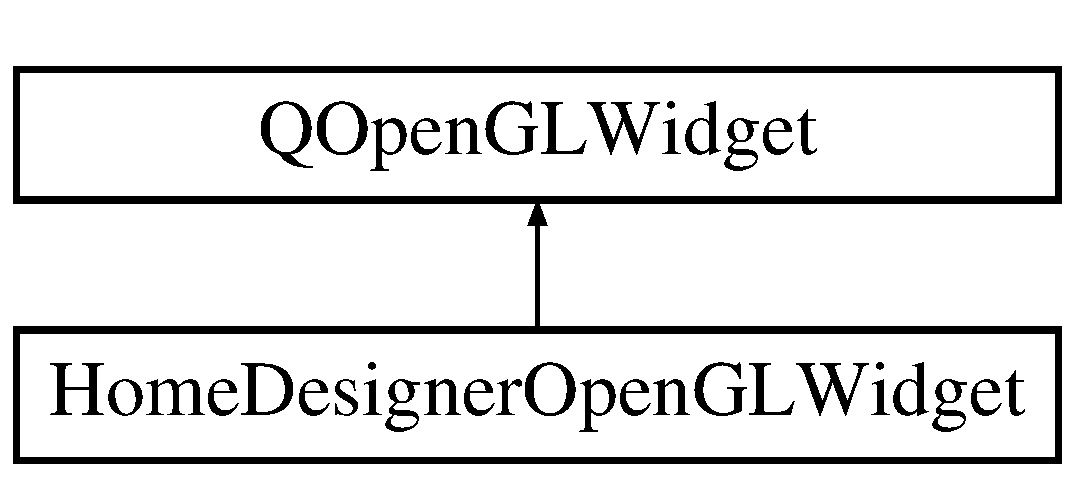
\includegraphics[height=2.000000cm]{class_home_designer_open_g_l_widget}
\end{center}
\end{figure}
\subsection*{Public Slots}
\begin{DoxyCompactItemize}
\item 
void \hyperlink{class_home_designer_open_g_l_widget_a17c63eebae07d7085b22aaf35746d59a}{On\+Move\+Selected\+Changed} (bool)
\begin{DoxyCompactList}\small\item\em On\+Move\+Selected\+Changed called when move selection changed. \end{DoxyCompactList}\item 
\hypertarget{class_home_designer_open_g_l_widget_ae46f16b4230341e60317f8cb9df8f53c}{}void \hyperlink{class_home_designer_open_g_l_widget_ae46f16b4230341e60317f8cb9df8f53c}{On\+Rotate\+Selected\+Changed} (bool)\label{class_home_designer_open_g_l_widget_ae46f16b4230341e60317f8cb9df8f53c}

\begin{DoxyCompactList}\small\item\em On\+Rotate\+Selected\+Changed called when rotation selection changed. \end{DoxyCompactList}\item 
\hypertarget{class_home_designer_open_g_l_widget_a3b689614d2a74932b75a7c18083b6c19}{}void \hyperlink{class_home_designer_open_g_l_widget_a3b689614d2a74932b75a7c18083b6c19}{On\+Scale\+Selected\+Changed} (bool)\label{class_home_designer_open_g_l_widget_a3b689614d2a74932b75a7c18083b6c19}

\begin{DoxyCompactList}\small\item\em On\+Scale\+Selected\+Changed called when scale selection changed. \end{DoxyCompactList}\item 
void \hyperlink{class_home_designer_open_g_l_widget_af6eec49ac86769b4fd23636743ac9150}{On\+Move\+Speed\+Changed} (int)
\begin{DoxyCompactList}\small\item\em On\+Move\+Speed\+Changed called when the move speed changed. \end{DoxyCompactList}\item 
\hypertarget{class_home_designer_open_g_l_widget_aeeb74ecdd39351f0229f28b394900581}{}void \hyperlink{class_home_designer_open_g_l_widget_aeeb74ecdd39351f0229f28b394900581}{On\+Rotate\+Speed\+Changed} (int)\label{class_home_designer_open_g_l_widget_aeeb74ecdd39351f0229f28b394900581}

\begin{DoxyCompactList}\small\item\em On\+Rotate\+Speed\+Changed calledon rotation speed changed. \end{DoxyCompactList}\item 
\hypertarget{class_home_designer_open_g_l_widget_a0f69f807f678735ce1d7ba41a7d495c3}{}void \hyperlink{class_home_designer_open_g_l_widget_a0f69f807f678735ce1d7ba41a7d495c3}{On\+Scale\+Speed\+Changed} (int)\label{class_home_designer_open_g_l_widget_a0f69f807f678735ce1d7ba41a7d495c3}

\begin{DoxyCompactList}\small\item\em On\+Scale\+Speed\+Changed called on scale speed changed. \end{DoxyCompactList}\item 
void \hyperlink{class_home_designer_open_g_l_widget_a4162c2eef3980d6a2f594c0c40bd169a}{On\+Load\+Model} (Q\+String model\+Attributes, G\+Lfloat initial\+Scale)
\begin{DoxyCompactList}\small\item\em On\+Load\+Model Loads a model from the file, setting its initial scale value. \end{DoxyCompactList}\item 
void \hyperlink{class_home_designer_open_g_l_widget_a0b14ecff70d70ec52b9ddced64ff4a2c}{On\+Operation\+Not\+Allowed} (Q\+String message)
\begin{DoxyCompactList}\small\item\em On\+Operation\+Not\+Allowed Displays a message when the operation (move, rotate, scale) isn\textquotesingle{}t allowed. \end{DoxyCompactList}\item 
void \hyperlink{class_home_designer_open_g_l_widget_ac9f66e0dc6799b7e48d6866d4322fa89}{On\+Operation\+Successful} ()
\begin{DoxyCompactList}\small\item\em On\+Operation\+Successful Restores the previous message in the status bar when the operation is successful. \end{DoxyCompactList}\item 
void \hyperlink{class_home_designer_open_g_l_widget_a18d664925e2c18855722e5300169f229}{On\+Change\+Room\+Wall\+Color} (Q\+Color color) const 
\begin{DoxyCompactList}\small\item\em On\+Change\+Room\+Wall\+Color Changes the wall color for the room. \end{DoxyCompactList}\item 
void \hyperlink{class_home_designer_open_g_l_widget_ad249a6ddc83b3eb0d119af8b0a694cac}{On\+Change\+Room\+Wall\+Texture} (Q\+String texture\+File\+Path) const 
\begin{DoxyCompactList}\small\item\em On\+Change\+Room\+Wall\+Texture Changes the wall texture. \end{DoxyCompactList}\item 
void \hyperlink{class_home_designer_open_g_l_widget_abe86574fe0641dd2d564a7964bc5ee8d}{On\+Change\+Room\+Floor\+Color} (Q\+Color color) const 
\begin{DoxyCompactList}\small\item\em On\+Change\+Room\+Floor\+Color changes the floor color. \end{DoxyCompactList}\item 
void \hyperlink{class_home_designer_open_g_l_widget_a99fb72c11d0a5a748e7342535219bf6e}{On\+Change\+Room\+Floor\+Texture} (Q\+String texture\+File\+Path) const 
\begin{DoxyCompactList}\small\item\em On\+Change\+Room\+Floor\+Texture changes the room texture. \end{DoxyCompactList}\end{DoxyCompactItemize}
\subsection*{Signals}
\begin{DoxyCompactItemize}
\item 
\hypertarget{class_home_designer_open_g_l_widget_ae8ccce3d055bc7c0889eea58c32315d8}{}void {\bfseries Exit} ()\label{class_home_designer_open_g_l_widget_ae8ccce3d055bc7c0889eea58c32315d8}

\item 
\hypertarget{class_home_designer_open_g_l_widget_acaf3c61231c51992ddc589ec4f87b080}{}void {\bfseries Display\+Message} (Q\+String message, int timeout)\label{class_home_designer_open_g_l_widget_acaf3c61231c51992ddc589ec4f87b080}

\item 
\hypertarget{class_home_designer_open_g_l_widget_a7da876eafb33c27ee6ea24100924a0ce}{}void {\bfseries Display\+Error} (Q\+String message)\label{class_home_designer_open_g_l_widget_a7da876eafb33c27ee6ea24100924a0ce}

\item 
\hypertarget{class_home_designer_open_g_l_widget_af43c80a3c488bf2a128c443ef7786782}{}void {\bfseries Clear\+Message} ()\label{class_home_designer_open_g_l_widget_af43c80a3c488bf2a128c443ef7786782}

\item 
\hypertarget{class_home_designer_open_g_l_widget_a9794810f40ecfb50cdd5bf4cdcf04cbe}{}void {\bfseries Axis\+Changed} (Axis old\+Axis, Axis axis)\label{class_home_designer_open_g_l_widget_a9794810f40ecfb50cdd5bf4cdcf04cbe}

\item 
\hypertarget{class_home_designer_open_g_l_widget_ab35b87b7e709ee647f6d44311d8942bf}{}void {\bfseries Collision\+Detected} (bool is\+Colliding)\label{class_home_designer_open_g_l_widget_ab35b87b7e709ee647f6d44311d8942bf}

\item 
\hypertarget{class_home_designer_open_g_l_widget_a231dd62d34d46dd13239c1cfa29a4292}{}void {\bfseries Update\+Status} (bool bounding\+Box, bool aa\+Boudning\+Box, bool world\+Axis, bool local\+Axis)\label{class_home_designer_open_g_l_widget_a231dd62d34d46dd13239c1cfa29a4292}

\end{DoxyCompactItemize}
\subsection*{Public Member Functions}
\begin{DoxyCompactItemize}
\item 
\hyperlink{class_home_designer_open_g_l_widget_a24232a9ac7981b4410a8fad3d3773ef5}{Home\+Designer\+Open\+G\+L\+Widget} (Q\+Widget $\ast$parent=nullptr)
\begin{DoxyCompactList}\small\item\em \hyperlink{class_home_designer_open_g_l_widget}{Home\+Designer\+Open\+G\+L\+Widget}. \end{DoxyCompactList}\item 
Axis \hyperlink{class_home_designer_open_g_l_widget_a9e4a4bfa55e86426d28ba0589035cec9}{Get\+Axis} () const 
\begin{DoxyCompactList}\small\item\em Get\+Axis. \end{DoxyCompactList}\item 
int \hyperlink{class_home_designer_open_g_l_widget_a766ed7c727cfbe473064fd244dede73d}{Get\+Move\+Speed} () const 
\begin{DoxyCompactList}\small\item\em Get\+Move\+Speed. \end{DoxyCompactList}\item 
void \hyperlink{class_home_designer_open_g_l_widget_a36605922069ae365da069207b97a058c}{Set\+Move\+Speed} (int speed)
\begin{DoxyCompactList}\small\item\em Set\+Move\+Speed. \end{DoxyCompactList}\item 
int \hyperlink{class_home_designer_open_g_l_widget_abdfd4baea7b439683ce0e87278335035}{Get\+Rotate\+Speed} () const 
\begin{DoxyCompactList}\small\item\em Get\+Rotate\+Speed. \end{DoxyCompactList}\item 
void \hyperlink{class_home_designer_open_g_l_widget_a8987eaba2c2dd6b0d5f1348c7a80db1c}{Set\+Rotate\+Speed} (int speed)
\begin{DoxyCompactList}\small\item\em Set\+Rotate\+Speed. \end{DoxyCompactList}\item 
int \hyperlink{class_home_designer_open_g_l_widget_a4eefb0e0be806ebd74ea6b13cfa941ee}{Get\+Scale\+Speed} () const 
\begin{DoxyCompactList}\small\item\em Get\+Scale\+Speed. \end{DoxyCompactList}\item 
void \hyperlink{class_home_designer_open_g_l_widget_a3bbe46ba314a8ef0a7a380fa7e8bbbdc}{Set\+Scale\+Speed} (int speed)
\begin{DoxyCompactList}\small\item\em Set\+Scale\+Speed. \end{DoxyCompactList}\end{DoxyCompactItemize}
\subsection*{Protected Member Functions}
\begin{DoxyCompactItemize}
\item 
void \hyperlink{class_home_designer_open_g_l_widget_a4222406ea010bada5b614f4aa9a408e3}{paint\+G\+L} () override
\begin{DoxyCompactList}\small\item\em paint\+G\+L Main loop of the application \end{DoxyCompactList}\item 
void \hyperlink{class_home_designer_open_g_l_widget_ab4d259ef3a1e4d80cc784f04d1e0da1f}{initialize\+G\+L} () override
\begin{DoxyCompactList}\small\item\em initialize\+G\+L Called when the widget is being initialized \end{DoxyCompactList}\item 
void \hyperlink{class_home_designer_open_g_l_widget_a9374ffef11f1f4be2eb7070e2a13ee65}{mouse\+Move\+Event} (Q\+Mouse\+Event $\ast$) override
\begin{DoxyCompactList}\small\item\em mouse\+Move\+Event Process mouse movement \end{DoxyCompactList}\item 
void \hyperlink{class_home_designer_open_g_l_widget_a44f26dde734bb6b1b4e30c4c2b2a6d9a}{key\+Press\+Event} (Q\+Key\+Event $\ast$) override
\begin{DoxyCompactList}\small\item\em key\+Press\+Event Process key press event \end{DoxyCompactList}\item 
void \hyperlink{class_home_designer_open_g_l_widget_aca029316bc95418bb9c6f8c372a74b0d}{key\+Release\+Event} (Q\+Key\+Event $\ast$) override
\begin{DoxyCompactList}\small\item\em key\+Release\+Event Reset pressed keys and modifiers, along with status bar message \end{DoxyCompactList}\item 
void \hyperlink{class_home_designer_open_g_l_widget_a89d62b03f15537ab73b7cd7af1346967}{mouse\+Press\+Event} (Q\+Mouse\+Event $\ast$) override
\begin{DoxyCompactList}\small\item\em mouse\+Press\+Event Keep track of mouse button(s) being pressed \end{DoxyCompactList}\item 
void \hyperlink{class_home_designer_open_g_l_widget_ab06746a2be49de22f1e3eac9cd34f49c}{mouse\+Release\+Event} (Q\+Mouse\+Event $\ast$) override
\begin{DoxyCompactList}\small\item\em mouse\+Release\+Event Reset mouse buttons and release mouse \end{DoxyCompactList}\item 
void \hyperlink{class_home_designer_open_g_l_widget_ac9a825748af7eaeb41bfe51fd5f99c1a}{wheel\+Event} (Q\+Wheel\+Event $\ast$) override
\begin{DoxyCompactList}\small\item\em wheel\+Event Allow Zoom in/out with mouse wheel \end{DoxyCompactList}\end{DoxyCompactItemize}


\subsection{Detailed Description}
The \hyperlink{class_home_designer_open_g_l_widget}{Home\+Designer\+Open\+G\+L\+Widget} class Which creates the view and projection matrices using perspective viewing,processes keyboard and mouse input allowing movement and zooming,Iterate through all models in the scene, draw them as necessary (including the bounding boxes and outline),collision detection. 

\subsection{Constructor \& Destructor Documentation}
\hypertarget{class_home_designer_open_g_l_widget_a24232a9ac7981b4410a8fad3d3773ef5}{}\index{Home\+Designer\+Open\+G\+L\+Widget@{Home\+Designer\+Open\+G\+L\+Widget}!Home\+Designer\+Open\+G\+L\+Widget@{Home\+Designer\+Open\+G\+L\+Widget}}
\index{Home\+Designer\+Open\+G\+L\+Widget@{Home\+Designer\+Open\+G\+L\+Widget}!Home\+Designer\+Open\+G\+L\+Widget@{Home\+Designer\+Open\+G\+L\+Widget}}
\subsubsection[{Home\+Designer\+Open\+G\+L\+Widget(\+Q\+Widget $\ast$parent=nullptr)}]{\setlength{\rightskip}{0pt plus 5cm}Home\+Designer\+Open\+G\+L\+Widget\+::\+Home\+Designer\+Open\+G\+L\+Widget (
\begin{DoxyParamCaption}
\item[{Q\+Widget $\ast$}]{parent = {\ttfamily nullptr}}
\end{DoxyParamCaption}
)\hspace{0.3cm}{\ttfamily [explicit]}}\label{class_home_designer_open_g_l_widget_a24232a9ac7981b4410a8fad3d3773ef5}


\hyperlink{class_home_designer_open_g_l_widget}{Home\+Designer\+Open\+G\+L\+Widget}. 


\begin{DoxyParams}{Parameters}
{\em parent} & \\
\hline
\end{DoxyParams}


\subsection{Member Function Documentation}
\hypertarget{class_home_designer_open_g_l_widget_a9e4a4bfa55e86426d28ba0589035cec9}{}\index{Home\+Designer\+Open\+G\+L\+Widget@{Home\+Designer\+Open\+G\+L\+Widget}!Get\+Axis@{Get\+Axis}}
\index{Get\+Axis@{Get\+Axis}!Home\+Designer\+Open\+G\+L\+Widget@{Home\+Designer\+Open\+G\+L\+Widget}}
\subsubsection[{Get\+Axis() const }]{\setlength{\rightskip}{0pt plus 5cm}Axis Home\+Designer\+Open\+G\+L\+Widget\+::\+Get\+Axis (
\begin{DoxyParamCaption}
{}
\end{DoxyParamCaption}
) const\hspace{0.3cm}{\ttfamily [inline]}}\label{class_home_designer_open_g_l_widget_a9e4a4bfa55e86426d28ba0589035cec9}


Get\+Axis. 

\begin{DoxyReturn}{Returns}

\end{DoxyReturn}
\hypertarget{class_home_designer_open_g_l_widget_a766ed7c727cfbe473064fd244dede73d}{}\index{Home\+Designer\+Open\+G\+L\+Widget@{Home\+Designer\+Open\+G\+L\+Widget}!Get\+Move\+Speed@{Get\+Move\+Speed}}
\index{Get\+Move\+Speed@{Get\+Move\+Speed}!Home\+Designer\+Open\+G\+L\+Widget@{Home\+Designer\+Open\+G\+L\+Widget}}
\subsubsection[{Get\+Move\+Speed() const }]{\setlength{\rightskip}{0pt plus 5cm}int Home\+Designer\+Open\+G\+L\+Widget\+::\+Get\+Move\+Speed (
\begin{DoxyParamCaption}
{}
\end{DoxyParamCaption}
) const\hspace{0.3cm}{\ttfamily [inline]}}\label{class_home_designer_open_g_l_widget_a766ed7c727cfbe473064fd244dede73d}


Get\+Move\+Speed. 

\begin{DoxyReturn}{Returns}

\end{DoxyReturn}
\hypertarget{class_home_designer_open_g_l_widget_abdfd4baea7b439683ce0e87278335035}{}\index{Home\+Designer\+Open\+G\+L\+Widget@{Home\+Designer\+Open\+G\+L\+Widget}!Get\+Rotate\+Speed@{Get\+Rotate\+Speed}}
\index{Get\+Rotate\+Speed@{Get\+Rotate\+Speed}!Home\+Designer\+Open\+G\+L\+Widget@{Home\+Designer\+Open\+G\+L\+Widget}}
\subsubsection[{Get\+Rotate\+Speed() const }]{\setlength{\rightskip}{0pt plus 5cm}int Home\+Designer\+Open\+G\+L\+Widget\+::\+Get\+Rotate\+Speed (
\begin{DoxyParamCaption}
{}
\end{DoxyParamCaption}
) const\hspace{0.3cm}{\ttfamily [inline]}}\label{class_home_designer_open_g_l_widget_abdfd4baea7b439683ce0e87278335035}


Get\+Rotate\+Speed. 

\begin{DoxyReturn}{Returns}

\end{DoxyReturn}
\hypertarget{class_home_designer_open_g_l_widget_a4eefb0e0be806ebd74ea6b13cfa941ee}{}\index{Home\+Designer\+Open\+G\+L\+Widget@{Home\+Designer\+Open\+G\+L\+Widget}!Get\+Scale\+Speed@{Get\+Scale\+Speed}}
\index{Get\+Scale\+Speed@{Get\+Scale\+Speed}!Home\+Designer\+Open\+G\+L\+Widget@{Home\+Designer\+Open\+G\+L\+Widget}}
\subsubsection[{Get\+Scale\+Speed() const }]{\setlength{\rightskip}{0pt plus 5cm}int Home\+Designer\+Open\+G\+L\+Widget\+::\+Get\+Scale\+Speed (
\begin{DoxyParamCaption}
{}
\end{DoxyParamCaption}
) const\hspace{0.3cm}{\ttfamily [inline]}}\label{class_home_designer_open_g_l_widget_a4eefb0e0be806ebd74ea6b13cfa941ee}


Get\+Scale\+Speed. 

\begin{DoxyReturn}{Returns}

\end{DoxyReturn}
\hypertarget{class_home_designer_open_g_l_widget_ab4d259ef3a1e4d80cc784f04d1e0da1f}{}\index{Home\+Designer\+Open\+G\+L\+Widget@{Home\+Designer\+Open\+G\+L\+Widget}!initialize\+G\+L@{initialize\+G\+L}}
\index{initialize\+G\+L@{initialize\+G\+L}!Home\+Designer\+Open\+G\+L\+Widget@{Home\+Designer\+Open\+G\+L\+Widget}}
\subsubsection[{initialize\+G\+L() override}]{\setlength{\rightskip}{0pt plus 5cm}void Home\+Designer\+Open\+G\+L\+Widget\+::initialize\+G\+L (
\begin{DoxyParamCaption}
{}
\end{DoxyParamCaption}
)\hspace{0.3cm}{\ttfamily [override]}, {\ttfamily [protected]}}\label{class_home_designer_open_g_l_widget_ab4d259ef3a1e4d80cc784f04d1e0da1f}


initialize\+G\+L Called when the widget is being initialized 

Called when the widget is being initialized \hypertarget{class_home_designer_open_g_l_widget_a44f26dde734bb6b1b4e30c4c2b2a6d9a}{}\index{Home\+Designer\+Open\+G\+L\+Widget@{Home\+Designer\+Open\+G\+L\+Widget}!key\+Press\+Event@{key\+Press\+Event}}
\index{key\+Press\+Event@{key\+Press\+Event}!Home\+Designer\+Open\+G\+L\+Widget@{Home\+Designer\+Open\+G\+L\+Widget}}
\subsubsection[{key\+Press\+Event(\+Q\+Key\+Event $\ast$) override}]{\setlength{\rightskip}{0pt plus 5cm}void Home\+Designer\+Open\+G\+L\+Widget\+::key\+Press\+Event (
\begin{DoxyParamCaption}
\item[{Q\+Key\+Event $\ast$}]{event}
\end{DoxyParamCaption}
)\hspace{0.3cm}{\ttfamily [override]}, {\ttfamily [protected]}}\label{class_home_designer_open_g_l_widget_a44f26dde734bb6b1b4e30c4c2b2a6d9a}


key\+Press\+Event Process key press event 

Process key press event \hypertarget{class_home_designer_open_g_l_widget_aca029316bc95418bb9c6f8c372a74b0d}{}\index{Home\+Designer\+Open\+G\+L\+Widget@{Home\+Designer\+Open\+G\+L\+Widget}!key\+Release\+Event@{key\+Release\+Event}}
\index{key\+Release\+Event@{key\+Release\+Event}!Home\+Designer\+Open\+G\+L\+Widget@{Home\+Designer\+Open\+G\+L\+Widget}}
\subsubsection[{key\+Release\+Event(\+Q\+Key\+Event $\ast$) override}]{\setlength{\rightskip}{0pt plus 5cm}void Home\+Designer\+Open\+G\+L\+Widget\+::key\+Release\+Event (
\begin{DoxyParamCaption}
\item[{Q\+Key\+Event $\ast$}]{event}
\end{DoxyParamCaption}
)\hspace{0.3cm}{\ttfamily [override]}, {\ttfamily [protected]}}\label{class_home_designer_open_g_l_widget_aca029316bc95418bb9c6f8c372a74b0d}


key\+Release\+Event Reset pressed keys and modifiers, along with status bar message 

Reset pressed keys and modifiers, along with status bar message \hypertarget{class_home_designer_open_g_l_widget_a9374ffef11f1f4be2eb7070e2a13ee65}{}\index{Home\+Designer\+Open\+G\+L\+Widget@{Home\+Designer\+Open\+G\+L\+Widget}!mouse\+Move\+Event@{mouse\+Move\+Event}}
\index{mouse\+Move\+Event@{mouse\+Move\+Event}!Home\+Designer\+Open\+G\+L\+Widget@{Home\+Designer\+Open\+G\+L\+Widget}}
\subsubsection[{mouse\+Move\+Event(\+Q\+Mouse\+Event $\ast$) override}]{\setlength{\rightskip}{0pt plus 5cm}void Home\+Designer\+Open\+G\+L\+Widget\+::mouse\+Move\+Event (
\begin{DoxyParamCaption}
\item[{Q\+Mouse\+Event $\ast$}]{event}
\end{DoxyParamCaption}
)\hspace{0.3cm}{\ttfamily [override]}, {\ttfamily [protected]}}\label{class_home_designer_open_g_l_widget_a9374ffef11f1f4be2eb7070e2a13ee65}


mouse\+Move\+Event Process mouse movement 

Process mouse movement \hypertarget{class_home_designer_open_g_l_widget_a89d62b03f15537ab73b7cd7af1346967}{}\index{Home\+Designer\+Open\+G\+L\+Widget@{Home\+Designer\+Open\+G\+L\+Widget}!mouse\+Press\+Event@{mouse\+Press\+Event}}
\index{mouse\+Press\+Event@{mouse\+Press\+Event}!Home\+Designer\+Open\+G\+L\+Widget@{Home\+Designer\+Open\+G\+L\+Widget}}
\subsubsection[{mouse\+Press\+Event(\+Q\+Mouse\+Event $\ast$) override}]{\setlength{\rightskip}{0pt plus 5cm}void Home\+Designer\+Open\+G\+L\+Widget\+::mouse\+Press\+Event (
\begin{DoxyParamCaption}
\item[{Q\+Mouse\+Event $\ast$}]{event}
\end{DoxyParamCaption}
)\hspace{0.3cm}{\ttfamily [override]}, {\ttfamily [protected]}}\label{class_home_designer_open_g_l_widget_a89d62b03f15537ab73b7cd7af1346967}


mouse\+Press\+Event Keep track of mouse button(s) being pressed 

Keep track of mouse button(s) being pressed \hypertarget{class_home_designer_open_g_l_widget_ab06746a2be49de22f1e3eac9cd34f49c}{}\index{Home\+Designer\+Open\+G\+L\+Widget@{Home\+Designer\+Open\+G\+L\+Widget}!mouse\+Release\+Event@{mouse\+Release\+Event}}
\index{mouse\+Release\+Event@{mouse\+Release\+Event}!Home\+Designer\+Open\+G\+L\+Widget@{Home\+Designer\+Open\+G\+L\+Widget}}
\subsubsection[{mouse\+Release\+Event(\+Q\+Mouse\+Event $\ast$) override}]{\setlength{\rightskip}{0pt plus 5cm}void Home\+Designer\+Open\+G\+L\+Widget\+::mouse\+Release\+Event (
\begin{DoxyParamCaption}
\item[{Q\+Mouse\+Event $\ast$}]{}
\end{DoxyParamCaption}
)\hspace{0.3cm}{\ttfamily [override]}, {\ttfamily [protected]}}\label{class_home_designer_open_g_l_widget_ab06746a2be49de22f1e3eac9cd34f49c}


mouse\+Release\+Event Reset mouse buttons and release mouse 

Reset mouse buttons and release mouse \hypertarget{class_home_designer_open_g_l_widget_abe86574fe0641dd2d564a7964bc5ee8d}{}\index{Home\+Designer\+Open\+G\+L\+Widget@{Home\+Designer\+Open\+G\+L\+Widget}!On\+Change\+Room\+Floor\+Color@{On\+Change\+Room\+Floor\+Color}}
\index{On\+Change\+Room\+Floor\+Color@{On\+Change\+Room\+Floor\+Color}!Home\+Designer\+Open\+G\+L\+Widget@{Home\+Designer\+Open\+G\+L\+Widget}}
\subsubsection[{On\+Change\+Room\+Floor\+Color}]{\setlength{\rightskip}{0pt plus 5cm}void Home\+Designer\+Open\+G\+L\+Widget\+::\+On\+Change\+Room\+Floor\+Color (
\begin{DoxyParamCaption}
\item[{Q\+Color}]{color}
\end{DoxyParamCaption}
) const\hspace{0.3cm}{\ttfamily [slot]}}\label{class_home_designer_open_g_l_widget_abe86574fe0641dd2d564a7964bc5ee8d}


On\+Change\+Room\+Floor\+Color changes the floor color. 


\begin{DoxyParams}{Parameters}
{\em color} & Changes the floor color \\
\hline
\end{DoxyParams}
\hypertarget{class_home_designer_open_g_l_widget_a99fb72c11d0a5a748e7342535219bf6e}{}\index{Home\+Designer\+Open\+G\+L\+Widget@{Home\+Designer\+Open\+G\+L\+Widget}!On\+Change\+Room\+Floor\+Texture@{On\+Change\+Room\+Floor\+Texture}}
\index{On\+Change\+Room\+Floor\+Texture@{On\+Change\+Room\+Floor\+Texture}!Home\+Designer\+Open\+G\+L\+Widget@{Home\+Designer\+Open\+G\+L\+Widget}}
\subsubsection[{On\+Change\+Room\+Floor\+Texture}]{\setlength{\rightskip}{0pt plus 5cm}void Home\+Designer\+Open\+G\+L\+Widget\+::\+On\+Change\+Room\+Floor\+Texture (
\begin{DoxyParamCaption}
\item[{Q\+String}]{texture\+File\+Path}
\end{DoxyParamCaption}
) const\hspace{0.3cm}{\ttfamily [slot]}}\label{class_home_designer_open_g_l_widget_a99fb72c11d0a5a748e7342535219bf6e}


On\+Change\+Room\+Floor\+Texture changes the room texture. 


\begin{DoxyParams}{Parameters}
{\em texture\+File\+Path} & Changes the floor texture \\
\hline
\end{DoxyParams}
\hypertarget{class_home_designer_open_g_l_widget_a18d664925e2c18855722e5300169f229}{}\index{Home\+Designer\+Open\+G\+L\+Widget@{Home\+Designer\+Open\+G\+L\+Widget}!On\+Change\+Room\+Wall\+Color@{On\+Change\+Room\+Wall\+Color}}
\index{On\+Change\+Room\+Wall\+Color@{On\+Change\+Room\+Wall\+Color}!Home\+Designer\+Open\+G\+L\+Widget@{Home\+Designer\+Open\+G\+L\+Widget}}
\subsubsection[{On\+Change\+Room\+Wall\+Color}]{\setlength{\rightskip}{0pt plus 5cm}void Home\+Designer\+Open\+G\+L\+Widget\+::\+On\+Change\+Room\+Wall\+Color (
\begin{DoxyParamCaption}
\item[{Q\+Color}]{color}
\end{DoxyParamCaption}
) const\hspace{0.3cm}{\ttfamily [slot]}}\label{class_home_designer_open_g_l_widget_a18d664925e2c18855722e5300169f229}


On\+Change\+Room\+Wall\+Color Changes the wall color for the room. 


\begin{DoxyParams}{Parameters}
{\em color} & Changes the wall color for the room \\
\hline
\end{DoxyParams}
\hypertarget{class_home_designer_open_g_l_widget_ad249a6ddc83b3eb0d119af8b0a694cac}{}\index{Home\+Designer\+Open\+G\+L\+Widget@{Home\+Designer\+Open\+G\+L\+Widget}!On\+Change\+Room\+Wall\+Texture@{On\+Change\+Room\+Wall\+Texture}}
\index{On\+Change\+Room\+Wall\+Texture@{On\+Change\+Room\+Wall\+Texture}!Home\+Designer\+Open\+G\+L\+Widget@{Home\+Designer\+Open\+G\+L\+Widget}}
\subsubsection[{On\+Change\+Room\+Wall\+Texture}]{\setlength{\rightskip}{0pt plus 5cm}void Home\+Designer\+Open\+G\+L\+Widget\+::\+On\+Change\+Room\+Wall\+Texture (
\begin{DoxyParamCaption}
\item[{Q\+String}]{texture\+File\+Path}
\end{DoxyParamCaption}
) const\hspace{0.3cm}{\ttfamily [slot]}}\label{class_home_designer_open_g_l_widget_ad249a6ddc83b3eb0d119af8b0a694cac}


On\+Change\+Room\+Wall\+Texture Changes the wall texture. 


\begin{DoxyParams}{Parameters}
{\em texture\+File\+Path} & Changes the wall texture \\
\hline
\end{DoxyParams}
\hypertarget{class_home_designer_open_g_l_widget_a4162c2eef3980d6a2f594c0c40bd169a}{}\index{Home\+Designer\+Open\+G\+L\+Widget@{Home\+Designer\+Open\+G\+L\+Widget}!On\+Load\+Model@{On\+Load\+Model}}
\index{On\+Load\+Model@{On\+Load\+Model}!Home\+Designer\+Open\+G\+L\+Widget@{Home\+Designer\+Open\+G\+L\+Widget}}
\subsubsection[{On\+Load\+Model}]{\setlength{\rightskip}{0pt plus 5cm}void Home\+Designer\+Open\+G\+L\+Widget\+::\+On\+Load\+Model (
\begin{DoxyParamCaption}
\item[{Q\+String}]{model\+Attributes, }
\item[{G\+Lfloat}]{initial\+Scale}
\end{DoxyParamCaption}
)\hspace{0.3cm}{\ttfamily [slot]}}\label{class_home_designer_open_g_l_widget_a4162c2eef3980d6a2f594c0c40bd169a}


On\+Load\+Model Loads a model from the file, setting its initial scale value. 


\begin{DoxyParams}{Parameters}
{\em model\+Attributes} & \\
\hline
{\em initial\+Scale} & Loads a model from the file, setting its initial scale value \\
\hline
\end{DoxyParams}
\hypertarget{class_home_designer_open_g_l_widget_a17c63eebae07d7085b22aaf35746d59a}{}\index{Home\+Designer\+Open\+G\+L\+Widget@{Home\+Designer\+Open\+G\+L\+Widget}!On\+Move\+Selected\+Changed@{On\+Move\+Selected\+Changed}}
\index{On\+Move\+Selected\+Changed@{On\+Move\+Selected\+Changed}!Home\+Designer\+Open\+G\+L\+Widget@{Home\+Designer\+Open\+G\+L\+Widget}}
\subsubsection[{On\+Move\+Selected\+Changed}]{\setlength{\rightskip}{0pt plus 5cm}void Home\+Designer\+Open\+G\+L\+Widget\+::\+On\+Move\+Selected\+Changed (
\begin{DoxyParamCaption}
\item[{bool}]{selected}
\end{DoxyParamCaption}
)\hspace{0.3cm}{\ttfamily [slot]}}\label{class_home_designer_open_g_l_widget_a17c63eebae07d7085b22aaf35746d59a}


On\+Move\+Selected\+Changed called when move selection changed. 

Called when the desired operation changes in the main window \hypertarget{class_home_designer_open_g_l_widget_af6eec49ac86769b4fd23636743ac9150}{}\index{Home\+Designer\+Open\+G\+L\+Widget@{Home\+Designer\+Open\+G\+L\+Widget}!On\+Move\+Speed\+Changed@{On\+Move\+Speed\+Changed}}
\index{On\+Move\+Speed\+Changed@{On\+Move\+Speed\+Changed}!Home\+Designer\+Open\+G\+L\+Widget@{Home\+Designer\+Open\+G\+L\+Widget}}
\subsubsection[{On\+Move\+Speed\+Changed}]{\setlength{\rightskip}{0pt plus 5cm}void Home\+Designer\+Open\+G\+L\+Widget\+::\+On\+Move\+Speed\+Changed (
\begin{DoxyParamCaption}
\item[{int}]{speed}
\end{DoxyParamCaption}
)\hspace{0.3cm}{\ttfamily [slot]}}\label{class_home_designer_open_g_l_widget_af6eec49ac86769b4fd23636743ac9150}


On\+Move\+Speed\+Changed called when the move speed changed. 

Called when the operation\textquotesingle{}s speed changes in the main window \hypertarget{class_home_designer_open_g_l_widget_a0b14ecff70d70ec52b9ddced64ff4a2c}{}\index{Home\+Designer\+Open\+G\+L\+Widget@{Home\+Designer\+Open\+G\+L\+Widget}!On\+Operation\+Not\+Allowed@{On\+Operation\+Not\+Allowed}}
\index{On\+Operation\+Not\+Allowed@{On\+Operation\+Not\+Allowed}!Home\+Designer\+Open\+G\+L\+Widget@{Home\+Designer\+Open\+G\+L\+Widget}}
\subsubsection[{On\+Operation\+Not\+Allowed}]{\setlength{\rightskip}{0pt plus 5cm}void Home\+Designer\+Open\+G\+L\+Widget\+::\+On\+Operation\+Not\+Allowed (
\begin{DoxyParamCaption}
\item[{Q\+String}]{message}
\end{DoxyParamCaption}
)\hspace{0.3cm}{\ttfamily [slot]}}\label{class_home_designer_open_g_l_widget_a0b14ecff70d70ec52b9ddced64ff4a2c}


On\+Operation\+Not\+Allowed Displays a message when the operation (move, rotate, scale) isn\textquotesingle{}t allowed. 


\begin{DoxyParams}{Parameters}
{\em message} & the message \\
\hline
\end{DoxyParams}
\hypertarget{class_home_designer_open_g_l_widget_ac9f66e0dc6799b7e48d6866d4322fa89}{}\index{Home\+Designer\+Open\+G\+L\+Widget@{Home\+Designer\+Open\+G\+L\+Widget}!On\+Operation\+Successful@{On\+Operation\+Successful}}
\index{On\+Operation\+Successful@{On\+Operation\+Successful}!Home\+Designer\+Open\+G\+L\+Widget@{Home\+Designer\+Open\+G\+L\+Widget}}
\subsubsection[{On\+Operation\+Successful}]{\setlength{\rightskip}{0pt plus 5cm}void Home\+Designer\+Open\+G\+L\+Widget\+::\+On\+Operation\+Successful (
\begin{DoxyParamCaption}
{}
\end{DoxyParamCaption}
)\hspace{0.3cm}{\ttfamily [slot]}}\label{class_home_designer_open_g_l_widget_ac9f66e0dc6799b7e48d6866d4322fa89}


On\+Operation\+Successful Restores the previous message in the status bar when the operation is successful. 

Restores the previous message in the status bar when the operation is successful \hypertarget{class_home_designer_open_g_l_widget_a4222406ea010bada5b614f4aa9a408e3}{}\index{Home\+Designer\+Open\+G\+L\+Widget@{Home\+Designer\+Open\+G\+L\+Widget}!paint\+G\+L@{paint\+G\+L}}
\index{paint\+G\+L@{paint\+G\+L}!Home\+Designer\+Open\+G\+L\+Widget@{Home\+Designer\+Open\+G\+L\+Widget}}
\subsubsection[{paint\+G\+L() override}]{\setlength{\rightskip}{0pt plus 5cm}void Home\+Designer\+Open\+G\+L\+Widget\+::paint\+G\+L (
\begin{DoxyParamCaption}
{}
\end{DoxyParamCaption}
)\hspace{0.3cm}{\ttfamily [override]}, {\ttfamily [protected]}}\label{class_home_designer_open_g_l_widget_a4222406ea010bada5b614f4aa9a408e3}


paint\+G\+L Main loop of the application 

Main loop of the application \hypertarget{class_home_designer_open_g_l_widget_a36605922069ae365da069207b97a058c}{}\index{Home\+Designer\+Open\+G\+L\+Widget@{Home\+Designer\+Open\+G\+L\+Widget}!Set\+Move\+Speed@{Set\+Move\+Speed}}
\index{Set\+Move\+Speed@{Set\+Move\+Speed}!Home\+Designer\+Open\+G\+L\+Widget@{Home\+Designer\+Open\+G\+L\+Widget}}
\subsubsection[{Set\+Move\+Speed(int speed)}]{\setlength{\rightskip}{0pt plus 5cm}void Home\+Designer\+Open\+G\+L\+Widget\+::\+Set\+Move\+Speed (
\begin{DoxyParamCaption}
\item[{int}]{speed}
\end{DoxyParamCaption}
)\hspace{0.3cm}{\ttfamily [inline]}}\label{class_home_designer_open_g_l_widget_a36605922069ae365da069207b97a058c}


Set\+Move\+Speed. 


\begin{DoxyParams}{Parameters}
{\em speed} & \\
\hline
\end{DoxyParams}
\hypertarget{class_home_designer_open_g_l_widget_a8987eaba2c2dd6b0d5f1348c7a80db1c}{}\index{Home\+Designer\+Open\+G\+L\+Widget@{Home\+Designer\+Open\+G\+L\+Widget}!Set\+Rotate\+Speed@{Set\+Rotate\+Speed}}
\index{Set\+Rotate\+Speed@{Set\+Rotate\+Speed}!Home\+Designer\+Open\+G\+L\+Widget@{Home\+Designer\+Open\+G\+L\+Widget}}
\subsubsection[{Set\+Rotate\+Speed(int speed)}]{\setlength{\rightskip}{0pt plus 5cm}void Home\+Designer\+Open\+G\+L\+Widget\+::\+Set\+Rotate\+Speed (
\begin{DoxyParamCaption}
\item[{int}]{speed}
\end{DoxyParamCaption}
)\hspace{0.3cm}{\ttfamily [inline]}}\label{class_home_designer_open_g_l_widget_a8987eaba2c2dd6b0d5f1348c7a80db1c}


Set\+Rotate\+Speed. 


\begin{DoxyParams}{Parameters}
{\em speed} & \\
\hline
\end{DoxyParams}
\hypertarget{class_home_designer_open_g_l_widget_a3bbe46ba314a8ef0a7a380fa7e8bbbdc}{}\index{Home\+Designer\+Open\+G\+L\+Widget@{Home\+Designer\+Open\+G\+L\+Widget}!Set\+Scale\+Speed@{Set\+Scale\+Speed}}
\index{Set\+Scale\+Speed@{Set\+Scale\+Speed}!Home\+Designer\+Open\+G\+L\+Widget@{Home\+Designer\+Open\+G\+L\+Widget}}
\subsubsection[{Set\+Scale\+Speed(int speed)}]{\setlength{\rightskip}{0pt plus 5cm}void Home\+Designer\+Open\+G\+L\+Widget\+::\+Set\+Scale\+Speed (
\begin{DoxyParamCaption}
\item[{int}]{speed}
\end{DoxyParamCaption}
)\hspace{0.3cm}{\ttfamily [inline]}}\label{class_home_designer_open_g_l_widget_a3bbe46ba314a8ef0a7a380fa7e8bbbdc}


Set\+Scale\+Speed. 


\begin{DoxyParams}{Parameters}
{\em speed} & \\
\hline
\end{DoxyParams}
\hypertarget{class_home_designer_open_g_l_widget_ac9a825748af7eaeb41bfe51fd5f99c1a}{}\index{Home\+Designer\+Open\+G\+L\+Widget@{Home\+Designer\+Open\+G\+L\+Widget}!wheel\+Event@{wheel\+Event}}
\index{wheel\+Event@{wheel\+Event}!Home\+Designer\+Open\+G\+L\+Widget@{Home\+Designer\+Open\+G\+L\+Widget}}
\subsubsection[{wheel\+Event(\+Q\+Wheel\+Event $\ast$) override}]{\setlength{\rightskip}{0pt plus 5cm}void Home\+Designer\+Open\+G\+L\+Widget\+::wheel\+Event (
\begin{DoxyParamCaption}
\item[{Q\+Wheel\+Event $\ast$}]{event}
\end{DoxyParamCaption}
)\hspace{0.3cm}{\ttfamily [override]}, {\ttfamily [protected]}}\label{class_home_designer_open_g_l_widget_ac9a825748af7eaeb41bfe51fd5f99c1a}


wheel\+Event Allow Zoom in/out with mouse wheel 

Zoom in/out with mouse wheel 

The documentation for this class was generated from the following files\+:\begin{DoxyCompactItemize}
\item 
Home\+Designer\+Open\+G\+L\+Widget.\+h\item 
Home\+Designer\+Open\+G\+L\+Widget.\+cpp\end{DoxyCompactItemize}

\hypertarget{class_main_window}{}\section{Main\+Window Class Reference}
\label{class_main_window}\index{Main\+Window@{Main\+Window}}


The \hyperlink{class_main_window}{Main\+Window} class sets the window size,layout,controls,colors.  




{\ttfamily \#include $<$Main\+Window.\+h$>$}

Inheritance diagram for Main\+Window\+:\begin{figure}[H]
\begin{center}
\leavevmode
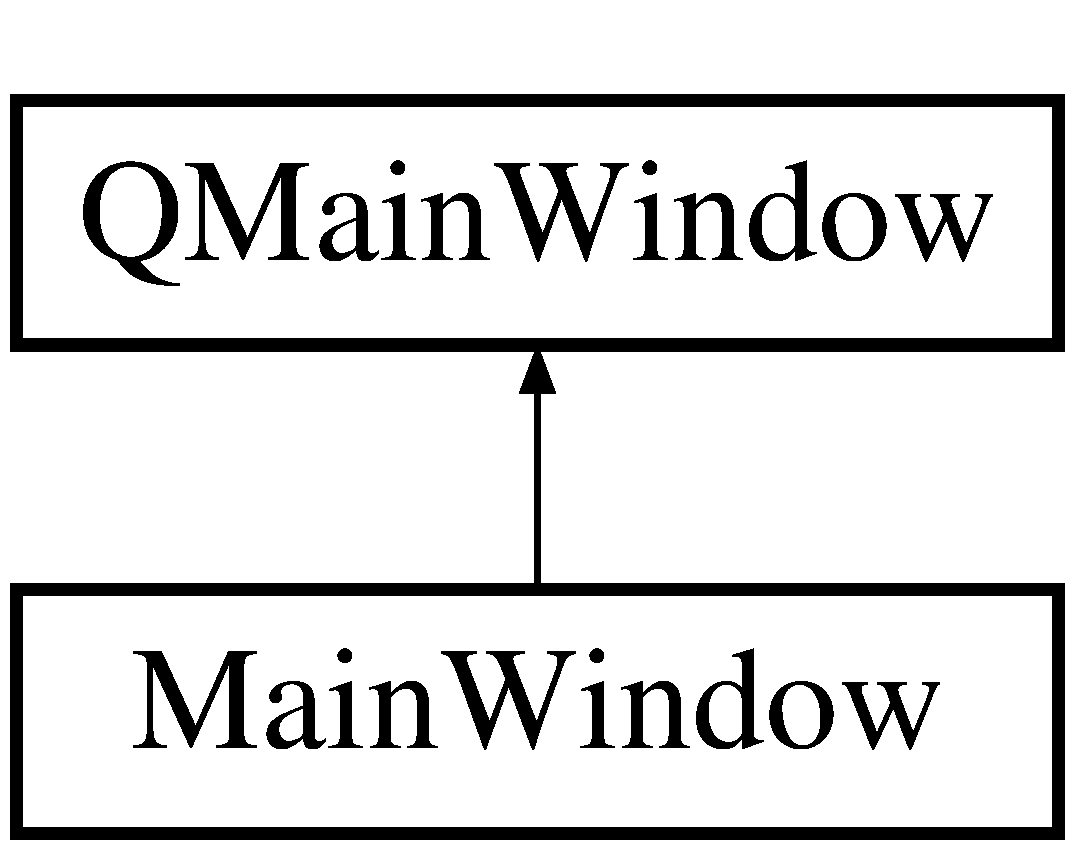
\includegraphics[height=2.000000cm]{class_main_window}
\end{center}
\end{figure}
\subsection*{Public Slots}
\begin{DoxyCompactItemize}
\item 
\hypertarget{class_main_window_abbfa33a7dbb6b6030aa117806e2a36dd}{}void {\bfseries On\+Change\+Buttons} (bool enable) const \label{class_main_window_abbfa33a7dbb6b6030aa117806e2a36dd}

\item 
\hypertarget{class_main_window_a28331903348b5b595826b88cc4ec8d65}{}void {\bfseries On\+Clear\+Message} () const \label{class_main_window_a28331903348b5b595826b88cc4ec8d65}

\item 
\hypertarget{class_main_window_a653116cd69aa29994ba258b6ae017aa1}{}void {\bfseries On\+Display\+Message} (Q\+String message, int timeout) const \label{class_main_window_a653116cd69aa29994ba258b6ae017aa1}

\item 
\hypertarget{class_main_window_ac6d6167eed399f17310482299e5600be}{}void {\bfseries On\+Display\+Error} (Q\+String message)\label{class_main_window_ac6d6167eed399f17310482299e5600be}

\item 
void \hyperlink{class_main_window_a1d28d674453152dece0a01678317b212}{On\+Update\+Status} (bool bounding\+Box, bool aa\+Boudning\+Box, bool world\+Axis, bool local\+Axis) const 
\begin{DoxyCompactList}\small\item\em On\+Update\+Status updates the status of the world axis, local axis ,bounding\+Box and aa\+Bounding\+Box, this is shows at the bottom of the screen. \end{DoxyCompactList}\item 
\hypertarget{class_main_window_aece5c2367706593bc723197c31dba842}{}void {\bfseries On\+Wall\+Color\+Button\+Clicked} ()\label{class_main_window_aece5c2367706593bc723197c31dba842}

\item 
\hypertarget{class_main_window_a128805a4505588f76abb1fb6897b75ab}{}void {\bfseries On\+Wall\+Texture\+Button\+Clicked} ()\label{class_main_window_a128805a4505588f76abb1fb6897b75ab}

\item 
\hypertarget{class_main_window_a518fec1c228151b47ed59a2f0a0ad7cf}{}void {\bfseries On\+Floor\+Color\+Button\+Clicked} ()\label{class_main_window_a518fec1c228151b47ed59a2f0a0ad7cf}

\item 
\hypertarget{class_main_window_a162c53dee72bb98df3255a4a3f30eb06}{}void {\bfseries On\+Floor\+Texture\+Button\+Clicked} ()\label{class_main_window_a162c53dee72bb98df3255a4a3f30eb06}

\end{DoxyCompactItemize}
\subsection*{Signals}
\begin{DoxyCompactItemize}
\item 
\hypertarget{class_main_window_a5a43372ffcce6aae9bb86d5b416854e1}{}void {\bfseries Change\+Room\+Wall\+Color} (Q\+Color color)\label{class_main_window_a5a43372ffcce6aae9bb86d5b416854e1}

\item 
\hypertarget{class_main_window_af86ec5a624baa391275a7b56e2729187}{}void {\bfseries Change\+Room\+Wall\+Texture} (Q\+String texture\+File\+Path)\label{class_main_window_af86ec5a624baa391275a7b56e2729187}

\item 
\hypertarget{class_main_window_a541dbc413da170b85d675b40dea1c049}{}void {\bfseries Change\+Room\+Floor\+Color} (Q\+Color color)\label{class_main_window_a541dbc413da170b85d675b40dea1c049}

\item 
\hypertarget{class_main_window_a4f913649fd4c09474b369faa60967d3b}{}void {\bfseries Change\+Room\+Floor\+Texture} (Q\+String texture\+File\+Path)\label{class_main_window_a4f913649fd4c09474b369faa60967d3b}

\end{DoxyCompactItemize}
\subsection*{Public Member Functions}
\begin{DoxyCompactItemize}
\item 
\hyperlink{class_main_window_a996c5a2b6f77944776856f08ec30858d}{Main\+Window} (Q\+Widget $\ast$parent=nullptr)
\begin{DoxyCompactList}\small\item\em \hyperlink{class_main_window}{Main\+Window} sets the size and controls and colors. \end{DoxyCompactList}\end{DoxyCompactItemize}


\subsection{Detailed Description}
The \hyperlink{class_main_window}{Main\+Window} class sets the window size,layout,controls,colors. 

\subsection{Constructor \& Destructor Documentation}
\hypertarget{class_main_window_a996c5a2b6f77944776856f08ec30858d}{}\index{Main\+Window@{Main\+Window}!Main\+Window@{Main\+Window}}
\index{Main\+Window@{Main\+Window}!Main\+Window@{Main\+Window}}
\subsubsection[{Main\+Window(\+Q\+Widget $\ast$parent=nullptr)}]{\setlength{\rightskip}{0pt plus 5cm}Main\+Window\+::\+Main\+Window (
\begin{DoxyParamCaption}
\item[{Q\+Widget $\ast$}]{parent = {\ttfamily nullptr}}
\end{DoxyParamCaption}
)\hspace{0.3cm}{\ttfamily [explicit]}}\label{class_main_window_a996c5a2b6f77944776856f08ec30858d}


\hyperlink{class_main_window}{Main\+Window} sets the size and controls and colors. 


\begin{DoxyParams}{Parameters}
{\em parent} & \\
\hline
\end{DoxyParams}


\subsection{Member Function Documentation}
\hypertarget{class_main_window_a1d28d674453152dece0a01678317b212}{}\index{Main\+Window@{Main\+Window}!On\+Update\+Status@{On\+Update\+Status}}
\index{On\+Update\+Status@{On\+Update\+Status}!Main\+Window@{Main\+Window}}
\subsubsection[{On\+Update\+Status}]{\setlength{\rightskip}{0pt plus 5cm}void Main\+Window\+::\+On\+Update\+Status (
\begin{DoxyParamCaption}
\item[{bool}]{bounding\+Box, }
\item[{bool}]{aa\+Boudning\+Box, }
\item[{bool}]{world\+Axis, }
\item[{bool}]{local\+Axis}
\end{DoxyParamCaption}
) const\hspace{0.3cm}{\ttfamily [slot]}}\label{class_main_window_a1d28d674453152dece0a01678317b212}


On\+Update\+Status updates the status of the world axis, local axis ,bounding\+Box and aa\+Bounding\+Box, this is shows at the bottom of the screen. 


\begin{DoxyParams}{Parameters}
{\em bounding\+Box} & \\
\hline
{\em aa\+Boudning\+Box} & \\
\hline
{\em world\+Axis} & \\
\hline
{\em local\+Axis} & \\
\hline
\end{DoxyParams}


The documentation for this class was generated from the following files\+:\begin{DoxyCompactItemize}
\item 
Main\+Window.\+h\item 
Main\+Window.\+cpp\end{DoxyCompactItemize}

\hypertarget{class_mesh}{}\section{Mesh Class Reference}
\label{class_mesh}\index{Mesh@{Mesh}}


The \hyperlink{class_mesh}{Mesh} class Provide the mesh with all the necessery variables vertices,indices, and textures and then draw the mesh.  




{\ttfamily \#include $<$Mesh.\+h$>$}

\subsection*{Public Member Functions}
\begin{DoxyCompactItemize}
\item 
\hyperlink{class_mesh_a9a4b7f1b6b50b9ad7e80c5d61d2b221b}{Mesh} (Q\+Open\+G\+L\+Widget $\ast$target\+Widget, vector$<$ \hyperlink{struct_vertex}{Vertex} $>$ vertices, vector$<$ G\+Luint $>$ indices, vector$<$ \hyperlink{struct_texture}{Texture} $>$ textures)
\begin{DoxyCompactList}\small\item\em \hyperlink{class_mesh}{Mesh} Provide the mesh with all the necessery data. \end{DoxyCompactList}\item 
\hypertarget{class_mesh_a7a01e69fcc56f348f7c91e1420b14e0e}{}G\+Luint {\bfseries Get\+Vao} () const \label{class_mesh_a7a01e69fcc56f348f7c91e1420b14e0e}

\item 
void \hyperlink{class_mesh_a143c8d7c179801c6377853db26d4a19f}{Draw} (\hyperlink{class_shader}{Shader} shader)
\begin{DoxyCompactList}\small\item\em Draw the drawing of the loaded mesh. \end{DoxyCompactList}\end{DoxyCompactItemize}
\subsection*{Public Attributes}
\begin{DoxyCompactItemize}
\item 
\hypertarget{class_mesh_abd28c74398f02e1afaa959c40bdd6df0}{}vector$<$ \hyperlink{struct_vertex}{Vertex} $>$ {\bfseries Vertices}\label{class_mesh_abd28c74398f02e1afaa959c40bdd6df0}

\item 
\hypertarget{class_mesh_ae293e39cb11bde8d46fe77ef622893bd}{}vector$<$ G\+Luint $>$ {\bfseries Indices}\label{class_mesh_ae293e39cb11bde8d46fe77ef622893bd}

\item 
\hypertarget{class_mesh_a10fa55f46fc6c5bb237525ed5343e73c}{}vector$<$ \hyperlink{struct_texture}{Texture} $>$ {\bfseries Textures}\label{class_mesh_a10fa55f46fc6c5bb237525ed5343e73c}

\end{DoxyCompactItemize}


\subsection{Detailed Description}
The \hyperlink{class_mesh}{Mesh} class Provide the mesh with all the necessery variables vertices,indices, and textures and then draw the mesh. 

\subsection{Constructor \& Destructor Documentation}
\hypertarget{class_mesh_a9a4b7f1b6b50b9ad7e80c5d61d2b221b}{}\index{Mesh@{Mesh}!Mesh@{Mesh}}
\index{Mesh@{Mesh}!Mesh@{Mesh}}
\subsubsection[{Mesh(\+Q\+Open\+G\+L\+Widget $\ast$target\+Widget, vector$<$ Vertex $>$ vertices, vector$<$ G\+Luint $>$ indices, vector$<$ Texture $>$ textures)}]{\setlength{\rightskip}{0pt plus 5cm}Mesh\+::\+Mesh (
\begin{DoxyParamCaption}
\item[{Q\+Open\+G\+L\+Widget $\ast$}]{target\+Widget, }
\item[{vector$<$ {\bf Vertex} $>$}]{vertices, }
\item[{vector$<$ G\+Luint $>$}]{indices, }
\item[{vector$<$ {\bf Texture} $>$}]{textures}
\end{DoxyParamCaption}
)\hspace{0.3cm}{\ttfamily [inline]}}\label{class_mesh_a9a4b7f1b6b50b9ad7e80c5d61d2b221b}


\hyperlink{class_mesh}{Mesh} Provide the mesh with all the necessery data. 


\begin{DoxyParams}{Parameters}
{\em target\+Widget} & the target width \\
\hline
{\em vertices} & the vertices \\
\hline
{\em indices} & the indices \\
\hline
{\em textures} & the texture \\
\hline
\end{DoxyParams}


\subsection{Member Function Documentation}
\hypertarget{class_mesh_a143c8d7c179801c6377853db26d4a19f}{}\index{Mesh@{Mesh}!Draw@{Draw}}
\index{Draw@{Draw}!Mesh@{Mesh}}
\subsubsection[{Draw(\+Shader shader)}]{\setlength{\rightskip}{0pt plus 5cm}void Mesh\+::\+Draw (
\begin{DoxyParamCaption}
\item[{{\bf Shader}}]{shader}
\end{DoxyParamCaption}
)\hspace{0.3cm}{\ttfamily [inline]}}\label{class_mesh_a143c8d7c179801c6377853db26d4a19f}


Draw the drawing of the loaded mesh. 


\begin{DoxyParams}{Parameters}
{\em shader} & \\
\hline
\end{DoxyParams}


The documentation for this class was generated from the following file\+:\begin{DoxyCompactItemize}
\item 
Mesh.\+h\end{DoxyCompactItemize}

\hypertarget{class_model}{}\section{Model Class Reference}
\label{class_model}\index{Model@{Model}}
\subsection*{Public Member Functions}
\begin{DoxyCompactItemize}
\item 
\hypertarget{class_model_a305581f2c1f2e77addbc7e436961c6dc}{}{\bfseries Model} (Q\+Open\+G\+L\+Widget $\ast$target\+Widget, string path)\label{class_model_a305581f2c1f2e77addbc7e436961c6dc}

\item 
\hypertarget{class_model_a9c66de8af7e48fefaccbb8a056ec3c1d}{}void {\bfseries Draw} (\hyperlink{class_shader}{Shader} \&shader)\label{class_model_a9c66de8af7e48fefaccbb8a056ec3c1d}

\item 
\hypertarget{class_model_a3ecdedb61ab3d622243ca0fcc900675f}{}void {\bfseries Draw\+Outline} (glm\+::mat4 \&model, \hyperlink{class_shader}{Shader} \&shader)\label{class_model_a3ecdedb61ab3d622243ca0fcc900675f}

\item 
\hypertarget{class_model_a9ea10d4e794c767d6fd2c3e69dde742a}{}void {\bfseries Draw\+Bounding\+Box} () const \label{class_model_a9ea10d4e794c767d6fd2c3e69dde742a}

\item 
\hypertarget{class_model_a2e44a9cc66044f1a0bec5c4590a4225c}{}void {\bfseries Draw\+Bounding\+Box} (const vector$<$ glm\+::vec3 $>$ \&vertices) const \label{class_model_a2e44a9cc66044f1a0bec5c4590a4225c}

\item 
\hypertarget{class_model_a3de6dceab0188445a152fcdf2fbe0cb9}{}vector$<$ \hyperlink{struct_texture}{Texture} $>$ {\bfseries Get\+Loaded\+Textures} () const \label{class_model_a3de6dceab0188445a152fcdf2fbe0cb9}

\item 
\hypertarget{class_model_adbef7b13fcb41b79702ddf0cddcd1300}{}vector$<$ \hyperlink{class_mesh}{Mesh} $>$ {\bfseries Get\+Meshes} () const \label{class_model_adbef7b13fcb41b79702ddf0cddcd1300}

\item 
\hypertarget{class_model_adb6de1964663b1d59182930047aa95ae}{}vector$<$ glm\+::vec3 $>$ {\bfseries Get\+Bounding\+Box\+Vertices} () const \label{class_model_adb6de1964663b1d59182930047aa95ae}

\item 
\hypertarget{class_model_a18dffdf7f50a87e32c9d8d8eea9a277a}{}string {\bfseries Get\+File\+Path} () const \label{class_model_a18dffdf7f50a87e32c9d8d8eea9a277a}

\end{DoxyCompactItemize}


The documentation for this class was generated from the following files\+:\begin{DoxyCompactItemize}
\item 
Model.\+h\item 
Model.\+cpp\end{DoxyCompactItemize}

\hypertarget{class_model_combo_box}{}\section{Model\+Combo\+Box Class Reference}
\label{class_model_combo_box}\index{Model\+Combo\+Box@{Model\+Combo\+Box}}


The \hyperlink{class_model_combo_box}{Model\+Combo\+Box} class Which will provide a list of models from which one can select to load.  




{\ttfamily \#include $<$Model\+Combo\+Box.\+h$>$}

Inheritance diagram for Model\+Combo\+Box\+:\begin{figure}[H]
\begin{center}
\leavevmode
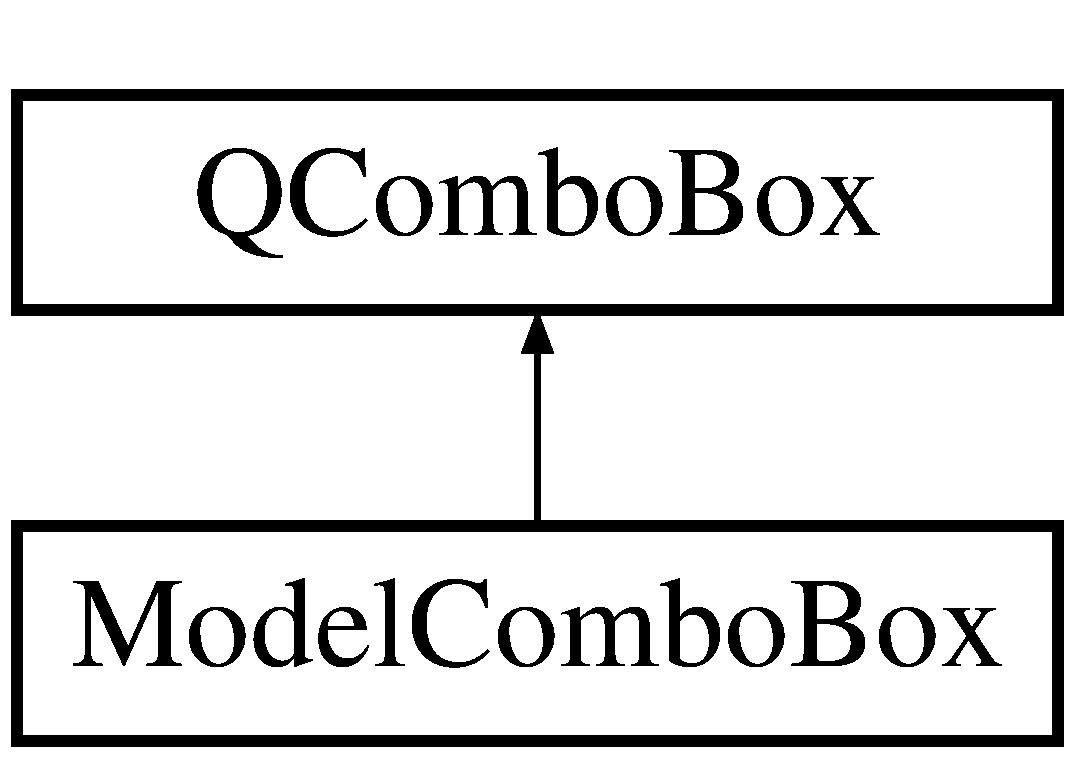
\includegraphics[height=2.000000cm]{class_model_combo_box}
\end{center}
\end{figure}
\subsection*{Classes}
\begin{DoxyCompactItemize}
\item 
class \hyperlink{class_model_combo_box_1_1_combo_box_delegate}{Combo\+Box\+Delegate}
\begin{DoxyCompactList}\small\item\em Solely used to draw the separator in our Combo\+Box. \end{DoxyCompactList}\end{DoxyCompactItemize}
\subsection*{Public Slots}
\begin{DoxyCompactItemize}
\item 
\hypertarget{class_model_combo_box_ac45a64e2c5ab7232c5dc99ef3eccd154}{}void \hyperlink{class_model_combo_box_ac45a64e2c5ab7232c5dc99ef3eccd154}{On\+Button\+Clicked} ()\label{class_model_combo_box_ac45a64e2c5ab7232c5dc99ef3eccd154}

\begin{DoxyCompactList}\small\item\em On\+Button\+Clicked when button is clicked in model exists it will be loaded. \end{DoxyCompactList}\end{DoxyCompactItemize}
\subsection*{Signals}
\begin{DoxyCompactItemize}
\item 
void \hyperlink{class_model_combo_box_aa521cbde3c50231f37ed0cf287bdcb1e}{Model\+Changed} (Q\+String model\+Attributes, G\+Lfloat initial\+Scale)
\begin{DoxyCompactList}\small\item\em Model\+Changed will determine when a model selection has changed and when we have loaded an initial scale. \end{DoxyCompactList}\end{DoxyCompactItemize}
\subsection*{Public Member Functions}
\begin{DoxyCompactItemize}
\item 
\hyperlink{class_model_combo_box_ac9c23e7ee48e1e04361c5f1bea08815c}{Model\+Combo\+Box} (Q\+Widget $\ast$parent=nullptr)
\begin{DoxyCompactList}\small\item\em \hyperlink{class_model_combo_box}{Model\+Combo\+Box} creates the model combo box. \end{DoxyCompactList}\end{DoxyCompactItemize}


\subsection{Detailed Description}
The \hyperlink{class_model_combo_box}{Model\+Combo\+Box} class Which will provide a list of models from which one can select to load. 

\subsection{Constructor \& Destructor Documentation}
\hypertarget{class_model_combo_box_ac9c23e7ee48e1e04361c5f1bea08815c}{}\index{Model\+Combo\+Box@{Model\+Combo\+Box}!Model\+Combo\+Box@{Model\+Combo\+Box}}
\index{Model\+Combo\+Box@{Model\+Combo\+Box}!Model\+Combo\+Box@{Model\+Combo\+Box}}
\subsubsection[{Model\+Combo\+Box(\+Q\+Widget $\ast$parent=nullptr)}]{\setlength{\rightskip}{0pt plus 5cm}Model\+Combo\+Box\+::\+Model\+Combo\+Box (
\begin{DoxyParamCaption}
\item[{Q\+Widget $\ast$}]{parent = {\ttfamily nullptr}}
\end{DoxyParamCaption}
)\hspace{0.3cm}{\ttfamily [explicit]}}\label{class_model_combo_box_ac9c23e7ee48e1e04361c5f1bea08815c}


\hyperlink{class_model_combo_box}{Model\+Combo\+Box} creates the model combo box. 


\begin{DoxyParams}{Parameters}
{\em parent} & the parent widget \\
\hline
\end{DoxyParams}


\subsection{Member Function Documentation}
\hypertarget{class_model_combo_box_aa521cbde3c50231f37ed0cf287bdcb1e}{}\index{Model\+Combo\+Box@{Model\+Combo\+Box}!Model\+Changed@{Model\+Changed}}
\index{Model\+Changed@{Model\+Changed}!Model\+Combo\+Box@{Model\+Combo\+Box}}
\subsubsection[{Model\+Changed}]{\setlength{\rightskip}{0pt plus 5cm}void Model\+Combo\+Box\+::\+Model\+Changed (
\begin{DoxyParamCaption}
\item[{Q\+String}]{model\+Attributes, }
\item[{G\+Lfloat}]{initial\+Scale}
\end{DoxyParamCaption}
)\hspace{0.3cm}{\ttfamily [signal]}}\label{class_model_combo_box_aa521cbde3c50231f37ed0cf287bdcb1e}


Model\+Changed will determine when a model selection has changed and when we have loaded an initial scale. 


\begin{DoxyParams}{Parameters}
{\em model\+Attributes} & the selected model from the combobox \\
\hline
{\em initial\+Scale} & usually 1 \\
\hline
\end{DoxyParams}


The documentation for this class was generated from the following files\+:\begin{DoxyCompactItemize}
\item 
Model\+Combo\+Box.\+h\item 
Model\+Combo\+Box.\+cpp\end{DoxyCompactItemize}

\hypertarget{class_model_container}{}\section{Model\+Container Class Reference}
\label{class_model_container}\index{Model\+Container@{Model\+Container}}


The \hyperlink{class_model_container}{Model\+Container} class.  




{\ttfamily \#include $<$Model\+Container.\+h$>$}

Inheritance diagram for Model\+Container\+:\begin{figure}[H]
\begin{center}
\leavevmode
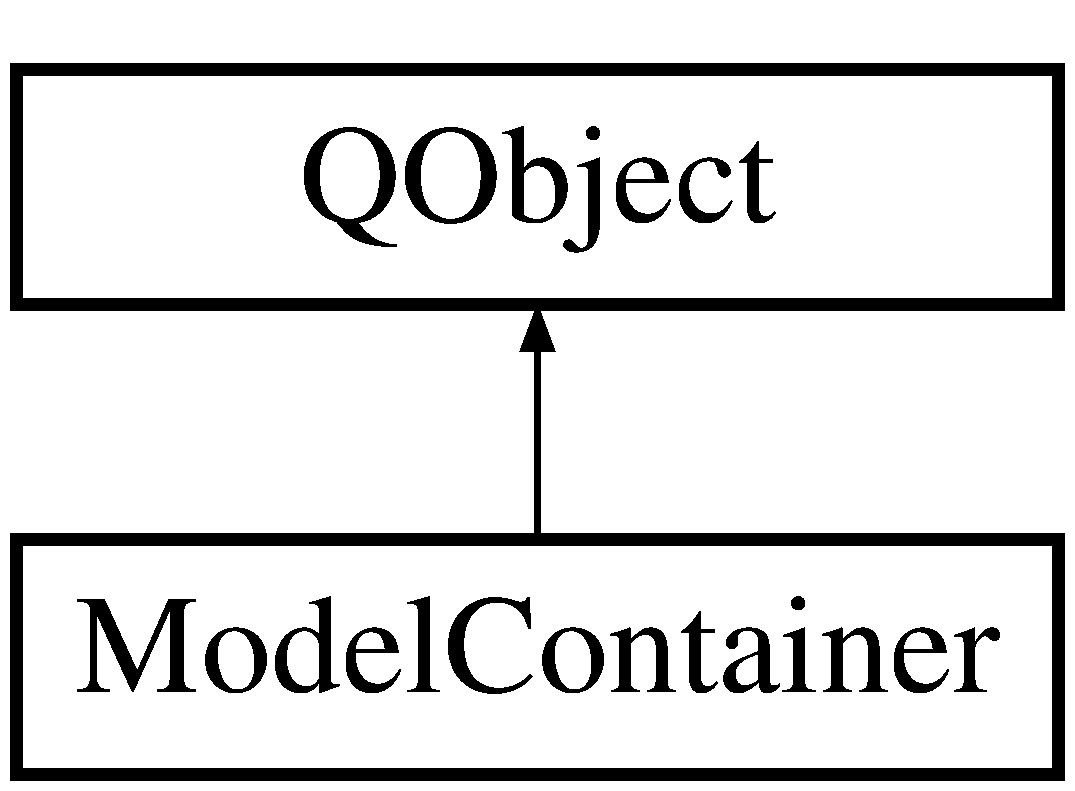
\includegraphics[height=2.000000cm]{class_model_container}
\end{center}
\end{figure}
\subsection*{Signals}
\begin{DoxyCompactItemize}
\item 
\hypertarget{class_model_container_a313ffe5493b9ed80d7a525f8530ff5f5}{}void {\bfseries Operation\+Not\+Allowed} (Q\+String message)\label{class_model_container_a313ffe5493b9ed80d7a525f8530ff5f5}

\item 
\hypertarget{class_model_container_af965a24540959f575f98f154269fafd6}{}void {\bfseries Operation\+Successful} ()\label{class_model_container_af965a24540959f575f98f154269fafd6}

\end{DoxyCompactItemize}
\subsection*{Public Member Functions}
\begin{DoxyCompactItemize}
\item 
\hyperlink{class_model_container_a5145271e175fb5434c5209d170a2749d}{Model\+Container} (\hyperlink{class_model}{Model} $\ast$model, G\+Lfloat initial\+Scale, \hyperlink{class_room}{Room} $\ast$room, Q\+Open\+G\+L\+Widget $\ast$target\+Widget)
\begin{DoxyCompactList}\small\item\em \hyperlink{class_model_container}{Model\+Container} Insert the model into the room provide initial scale factor and target width. Check that it fits into the room and that it is currently not colliding with anything. \end{DoxyCompactList}\item 
\hypertarget{class_model_container_ad403022f0e44b40ae6576b1c9454263e}{}G\+Lfloat {\bfseries Get\+Scale\+Factor} () const \label{class_model_container_ad403022f0e44b40ae6576b1c9454263e}

\item 
\hypertarget{class_model_container_ae859dd4743c5c4dcd3ed4044dfe60ffe}{}glm\+::vec3 {\bfseries Get\+Scale\+Vector} () const \label{class_model_container_ae859dd4743c5c4dcd3ed4044dfe60ffe}

\item 
\hypertarget{class_model_container_ad76f4a36da8b3696089f2843382cf9fb}{}glm\+::vec3 {\bfseries Get\+Translation\+Vector} () const \label{class_model_container_ad76f4a36da8b3696089f2843382cf9fb}

\item 
\hypertarget{class_model_container_a1346377aa22a8e763475cc868e7b085c}{}glm\+::vec3 {\bfseries Get\+Rotation\+Angles} () const \label{class_model_container_a1346377aa22a8e763475cc868e7b085c}

\item 
\hypertarget{class_model_container_a14d2a1daa39d7f051a0022b577b8759e}{}vector$<$ glm\+::vec3 $>$ const \& {\bfseries Get\+Bounding\+Box\+Vertices} () const \label{class_model_container_a14d2a1daa39d7f051a0022b577b8759e}

\item 
\hypertarget{class_model_container_a5d5e757812e3c6d26b7217618f52680d}{}glm\+::vec3 {\bfseries Get\+Minimum\+Vertices} () const \label{class_model_container_a5d5e757812e3c6d26b7217618f52680d}

\item 
\hypertarget{class_model_container_af5b5265648933d3effb2e75c69412290}{}glm\+::vec3 {\bfseries Get\+Maximum\+Vertices} () const \label{class_model_container_af5b5265648933d3effb2e75c69412290}

\item 
\hypertarget{class_model_container_ac842121f3683631e63d232784841b1ea}{}glm\+::vec3 {\bfseries get\+Model\+Container\+Center} () const \label{class_model_container_ac842121f3683631e63d232784841b1ea}

\item 
\hypertarget{class_model_container_a277b409fafa9f2e51eca3ceaf05842b5}{}glm\+::mat4 {\bfseries Get\+Model\+Matrix} () const \label{class_model_container_a277b409fafa9f2e51eca3ceaf05842b5}

\item 
\hypertarget{class_model_container_adf273cf3b683f5f5452414d473afe2cb}{}void {\bfseries Set\+Initial\+Scale} (G\+Lfloat initial\+Scale)\label{class_model_container_adf273cf3b683f5f5452414d473afe2cb}

\item 
\hypertarget{class_model_container_a1ca63a7256501991de59f33452a20aae}{}void {\bfseries Set\+Initial\+Translate\+Vector} (glm\+::vec3 initial\+Translate\+Vector)\label{class_model_container_a1ca63a7256501991de59f33452a20aae}

\item 
\hypertarget{class_model_container_a29ae098cea587ffbd6595427045971b3}{}void {\bfseries Set\+Initial\+Rotation\+Angles} (glm\+::vec3 initial\+Rotation\+Angles)\label{class_model_container_a29ae098cea587ffbd6595427045971b3}

\item 
\hypertarget{class_model_container_a75175aeab083d162034b357205270759}{}Location {\bfseries Get\+Bounded\+Wall} () const \label{class_model_container_a75175aeab083d162034b357205270759}

\item 
\hypertarget{class_model_container_ae38be381c9c05dd5b6d505d1830d4264}{}void {\bfseries Set\+Bounded\+Wall} (Location wall\+Location)\label{class_model_container_ae38be381c9c05dd5b6d505d1830d4264}

\item 
\hypertarget{class_model_container_a0163bcb5b8ff80f52cfb043ec0f3aa63}{}\hyperlink{class_model}{Model} $\ast$ {\bfseries Get\+Model} () const \label{class_model_container_a0163bcb5b8ff80f52cfb043ec0f3aa63}

\item 
\hypertarget{class_model_container_a9df86e06bcda6af814008c136b1023e8}{}glm\+::mat4 {\bfseries Get\+Transform\+Matrix} () const \label{class_model_container_a9df86e06bcda6af814008c136b1023e8}

\item 
\hypertarget{class_model_container_a9f7fc23d5b09502dbb442b3f65c294ce}{}glm\+::mat4 \hyperlink{class_model_container_a9f7fc23d5b09502dbb442b3f65c294ce}{Get\+Transform\+Rotate\+Matrix} () const \label{class_model_container_a9f7fc23d5b09502dbb442b3f65c294ce}

\begin{DoxyCompactList}\small\item\em Get the transform-\/rotate matrix. \end{DoxyCompactList}\item 
\hypertarget{class_model_container_a2a91fc30179a9da8195e704bcf6bb179}{}void {\bfseries Set\+Projection\+Matrix} (glm\+::mat4 \&projection)\label{class_model_container_a2a91fc30179a9da8195e704bcf6bb179}

\item 
\hypertarget{class_model_container_a14648db778747762f55ad52396225efa}{}void {\bfseries Set\+View\+Matrix} (glm\+::mat4 \&view)\label{class_model_container_a14648db778747762f55ad52396225efa}

\item 
\hypertarget{class_model_container_afb5c293199114bcd6da5bea8b964b732}{}void {\bfseries Set\+Translation\+Bound} (glm\+::vec3 translation\+Bound)\label{class_model_container_afb5c293199114bcd6da5bea8b964b732}

\item 
\hypertarget{class_model_container_a9d5ae2036e06e9230942fb45b8f5156a}{}void {\bfseries Set\+Rotation\+Bound} (glm\+::vec3 rotation\+Bound)\label{class_model_container_a9d5ae2036e06e9230942fb45b8f5156a}

\item 
\hypertarget{class_model_container_a9bc78b840b5bb544db86cb5956b17a12}{}void {\bfseries Set\+Scale\+Bound} (glm\+::vec3 scale\+Bound)\label{class_model_container_a9bc78b840b5bb544db86cb5956b17a12}

\item 
void \hyperlink{class_model_container_ac8d13143fdc69ce02d2539dd677bc3db}{Scale\+By} (G\+Lfloat scale\+Factor)
\begin{DoxyCompactList}\small\item\em Scale\+By. \end{DoxyCompactList}\item 
void \hyperlink{class_model_container_a40a0e922136e185a3808dac214d9cea8}{Rotate\+By} (glm\+::vec3 angles)
\begin{DoxyCompactList}\small\item\em Rotate\+By. \end{DoxyCompactList}\item 
void \hyperlink{class_model_container_ac33db8cfd1cac6742735dcc0226feff0}{Translate\+By} (glm\+::vec3 translate\+Vector)
\begin{DoxyCompactList}\small\item\em Translate\+By. \end{DoxyCompactList}\item 
\hypertarget{class_model_container_a349647d2eccc777419ff6eeb8edeff90}{}bool {\bfseries Is\+Selected} () const \label{class_model_container_a349647d2eccc777419ff6eeb8edeff90}

\item 
\hypertarget{class_model_container_a56c9edb4f2eb179a213e639dbaa05c9e}{}bool {\bfseries Set\+Selected} (bool selected)\label{class_model_container_a56c9edb4f2eb179a213e639dbaa05c9e}

\item 
\hypertarget{class_model_container_ad772dd3ae73fa1f3237c83e97a5fc80b}{}bool {\bfseries Is\+Colliding} () const \label{class_model_container_ad772dd3ae73fa1f3237c83e97a5fc80b}

\item 
void \hyperlink{class_model_container_a9d6352f35e74be676bf923d38ec0b24c}{Draw\+Model} (\hyperlink{class_shader}{Shader} \&shader, \hyperlink{class_shader}{Shader} \&outline\+Shader, int index)
\begin{DoxyCompactList}\small\item\em Draw\+Model. \end{DoxyCompactList}\item 
void \hyperlink{class_model_container_a4f73480431ca9bca8cbcdac87ef1d055}{Draw\+Model\+Bounding\+Box} (\hyperlink{class_shader}{Shader} \&shader)
\begin{DoxyCompactList}\small\item\em Draw\+Model\+Bounding\+Box. \end{DoxyCompactList}\item 
void \hyperlink{class_model_container_a6048f0f26f86025c6854bf42d7c5cc19}{Draw\+A\+A\+Boudning\+Box} (\hyperlink{class_shader}{Shader} \&shader)
\begin{DoxyCompactList}\small\item\em Draw\+A\+A\+Boudning\+Box. \end{DoxyCompactList}\item 
\hypertarget{class_model_container_aff6393883a26f3d71476e24e34f58852}{}void {\bfseries Reset} ()\label{class_model_container_aff6393883a26f3d71476e24e34f58852}

\item 
\hypertarget{class_model_container_a84dee4d7878153ecd2971427b2dd4c87}{}bool {\bfseries Is\+Inside\+Room} () const \label{class_model_container_a84dee4d7878153ecd2971427b2dd4c87}

\end{DoxyCompactItemize}


\subsection{Detailed Description}
The \hyperlink{class_model_container}{Model\+Container} class. 

\subsection{Constructor \& Destructor Documentation}
\hypertarget{class_model_container_a5145271e175fb5434c5209d170a2749d}{}\index{Model\+Container@{Model\+Container}!Model\+Container@{Model\+Container}}
\index{Model\+Container@{Model\+Container}!Model\+Container@{Model\+Container}}
\subsubsection[{Model\+Container(\+Model $\ast$model, G\+Lfloat initial\+Scale, Room $\ast$room, Q\+Open\+G\+L\+Widget $\ast$target\+Widget)}]{\setlength{\rightskip}{0pt plus 5cm}Model\+Container\+::\+Model\+Container (
\begin{DoxyParamCaption}
\item[{{\bf Model} $\ast$}]{model, }
\item[{G\+Lfloat}]{initial\+Scale, }
\item[{{\bf Room} $\ast$}]{room, }
\item[{Q\+Open\+G\+L\+Widget $\ast$}]{target\+Widget}
\end{DoxyParamCaption}
)}\label{class_model_container_a5145271e175fb5434c5209d170a2749d}


\hyperlink{class_model_container}{Model\+Container} Insert the model into the room provide initial scale factor and target width. Check that it fits into the room and that it is currently not colliding with anything. 


\begin{DoxyParams}{Parameters}
{\em model} & \\
\hline
{\em initial\+Scale} & \\
\hline
{\em room} & \\
\hline
{\em target\+Widget} & \\
\hline
\end{DoxyParams}


\subsection{Member Function Documentation}
\hypertarget{class_model_container_a6048f0f26f86025c6854bf42d7c5cc19}{}\index{Model\+Container@{Model\+Container}!Draw\+A\+A\+Boudning\+Box@{Draw\+A\+A\+Boudning\+Box}}
\index{Draw\+A\+A\+Boudning\+Box@{Draw\+A\+A\+Boudning\+Box}!Model\+Container@{Model\+Container}}
\subsubsection[{Draw\+A\+A\+Boudning\+Box(\+Shader \&shader)}]{\setlength{\rightskip}{0pt plus 5cm}void Model\+Container\+::\+Draw\+A\+A\+Boudning\+Box (
\begin{DoxyParamCaption}
\item[{{\bf Shader} \&}]{shader}
\end{DoxyParamCaption}
)}\label{class_model_container_a6048f0f26f86025c6854bf42d7c5cc19}


Draw\+A\+A\+Boudning\+Box. 


\begin{DoxyParams}{Parameters}
{\em shader} & \\
\hline
\end{DoxyParams}
\hypertarget{class_model_container_a9d6352f35e74be676bf923d38ec0b24c}{}\index{Model\+Container@{Model\+Container}!Draw\+Model@{Draw\+Model}}
\index{Draw\+Model@{Draw\+Model}!Model\+Container@{Model\+Container}}
\subsubsection[{Draw\+Model(\+Shader \&shader, Shader \&outline\+Shader, int index)}]{\setlength{\rightskip}{0pt plus 5cm}void Model\+Container\+::\+Draw\+Model (
\begin{DoxyParamCaption}
\item[{{\bf Shader} \&}]{shader, }
\item[{{\bf Shader} \&}]{outline\+Shader, }
\item[{int}]{index}
\end{DoxyParamCaption}
)}\label{class_model_container_a9d6352f35e74be676bf923d38ec0b24c}


Draw\+Model. 


\begin{DoxyParams}{Parameters}
{\em shader} & \\
\hline
{\em outline\+Shader} & \\
\hline
{\em index} & \\
\hline
\end{DoxyParams}
\hypertarget{class_model_container_a4f73480431ca9bca8cbcdac87ef1d055}{}\index{Model\+Container@{Model\+Container}!Draw\+Model\+Bounding\+Box@{Draw\+Model\+Bounding\+Box}}
\index{Draw\+Model\+Bounding\+Box@{Draw\+Model\+Bounding\+Box}!Model\+Container@{Model\+Container}}
\subsubsection[{Draw\+Model\+Bounding\+Box(\+Shader \&shader)}]{\setlength{\rightskip}{0pt plus 5cm}void Model\+Container\+::\+Draw\+Model\+Bounding\+Box (
\begin{DoxyParamCaption}
\item[{{\bf Shader} \&}]{shader}
\end{DoxyParamCaption}
)}\label{class_model_container_a4f73480431ca9bca8cbcdac87ef1d055}


Draw\+Model\+Bounding\+Box. 


\begin{DoxyParams}{Parameters}
{\em shader} & \\
\hline
\end{DoxyParams}
\hypertarget{class_model_container_a40a0e922136e185a3808dac214d9cea8}{}\index{Model\+Container@{Model\+Container}!Rotate\+By@{Rotate\+By}}
\index{Rotate\+By@{Rotate\+By}!Model\+Container@{Model\+Container}}
\subsubsection[{Rotate\+By(glm\+::vec3 angles)}]{\setlength{\rightskip}{0pt plus 5cm}void Model\+Container\+::\+Rotate\+By (
\begin{DoxyParamCaption}
\item[{glm\+::vec3}]{angles}
\end{DoxyParamCaption}
)}\label{class_model_container_a40a0e922136e185a3808dac214d9cea8}


Rotate\+By. 


\begin{DoxyParams}{Parameters}
{\em angles} & \\
\hline
\end{DoxyParams}
\hypertarget{class_model_container_ac8d13143fdc69ce02d2539dd677bc3db}{}\index{Model\+Container@{Model\+Container}!Scale\+By@{Scale\+By}}
\index{Scale\+By@{Scale\+By}!Model\+Container@{Model\+Container}}
\subsubsection[{Scale\+By(\+G\+Lfloat scale\+Factor)}]{\setlength{\rightskip}{0pt plus 5cm}void Model\+Container\+::\+Scale\+By (
\begin{DoxyParamCaption}
\item[{G\+Lfloat}]{scale\+Factor}
\end{DoxyParamCaption}
)}\label{class_model_container_ac8d13143fdc69ce02d2539dd677bc3db}


Scale\+By. 


\begin{DoxyParams}{Parameters}
{\em scale\+Factor} & \\
\hline
\end{DoxyParams}
\hypertarget{class_model_container_ac33db8cfd1cac6742735dcc0226feff0}{}\index{Model\+Container@{Model\+Container}!Translate\+By@{Translate\+By}}
\index{Translate\+By@{Translate\+By}!Model\+Container@{Model\+Container}}
\subsubsection[{Translate\+By(glm\+::vec3 translate\+Vector)}]{\setlength{\rightskip}{0pt plus 5cm}void Model\+Container\+::\+Translate\+By (
\begin{DoxyParamCaption}
\item[{glm\+::vec3}]{translate\+Vector}
\end{DoxyParamCaption}
)}\label{class_model_container_ac33db8cfd1cac6742735dcc0226feff0}


Translate\+By. 


\begin{DoxyParams}{Parameters}
{\em translate\+Vector} & \\
\hline
\end{DoxyParams}


The documentation for this class was generated from the following files\+:\begin{DoxyCompactItemize}
\item 
Model\+Container.\+h\item 
Model\+Container.\+cpp\end{DoxyCompactItemize}

\hypertarget{class_room}{}\section{Room Class Reference}
\label{class_room}\index{Room@{Room}}
\subsection*{Public Member Functions}
\begin{DoxyCompactItemize}
\item 
\hyperlink{class_room_a7b347765e9501c064013258629b4de19}{Room} (Q\+Open\+G\+L\+Widget $\ast$target\+Widget, G\+Lfloat room\+Width, glm\+::vec3 wall\+Color, glm\+::vec3 floor\+Color)
\item 
\hypertarget{class_room_ae621e50fd276c68af137ab02666dcee8}{}\hyperlink{class_floor}{Floor} $\ast$ {\bfseries Get\+Floor} () const \label{class_room_ae621e50fd276c68af137ab02666dcee8}

\item 
\hypertarget{class_room_a99f66c521d11492e4699a8f9aca6fa25}{}vector$<$ shared\+\_\+ptr$<$ \hyperlink{class_wall}{Wall} $>$ $>$ {\bfseries Get\+Walls} () const \label{class_room_a99f66c521d11492e4699a8f9aca6fa25}

\item 
void \hyperlink{class_room_a0fee2b31c00e8965934ddb0cba8dab9f}{Set\+Wall\+Color} (glm\+::vec3 wall\+Color)
\item 
\hypertarget{class_room_a4a5c9022582a2acaa29196a45c864e6c}{}glm\+::vec3 {\bfseries Get\+Wall\+Color} () const \label{class_room_a4a5c9022582a2acaa29196a45c864e6c}

\item 
void \hyperlink{class_room_a47df29040992bde5444c485b0b942aad}{Set\+Floor\+Color} (glm\+::vec3 floor\+Color)
\item 
\hypertarget{class_room_a92d642a94fd6a2b65094501e17559b48}{}glm\+::vec3 {\bfseries Get\+Floor\+Color} () const \label{class_room_a92d642a94fd6a2b65094501e17559b48}

\item 
void \hyperlink{class_room_ab0f733f37df1351b30573dcc8e13a18d}{Set\+Wall\+Texture} (string wall\+Texture)
\item 
\hypertarget{class_room_a9767bef2a8361a6654d77d522bee77e7}{}string {\bfseries Get\+Wall\+Texture} () const \label{class_room_a9767bef2a8361a6654d77d522bee77e7}

\item 
void \hyperlink{class_room_af6104c7b967af777bc8b054179f43829}{Set\+Floor\+Texture} (string floor\+Texture)
\item 
\hypertarget{class_room_a604d2069548456e15fc537b56900a4e0}{}string {\bfseries Get\+Floor\+Texture} () const \label{class_room_a604d2069548456e15fc537b56900a4e0}

\item 
glm\+::vec3 \hyperlink{class_room_a2a11f153f356dca23b40cd8147150cb9}{Get\+Minimum\+Coordinates} () const 
\item 
glm\+::vec3 \hyperlink{class_room_a1303223ef4eb22b9580148204f1de346}{Get\+Maximum\+Coordinates} () const 
\item 
void \hyperlink{class_room_a013a7a067df01681afa7b8bfda69e48e}{Draw} (glm\+::mat4 const \&view, glm\+::mat4 const \&projection) const 
\item 
void \hyperlink{class_room_afc80f1892eaa6db27ac526b4ec77d8bd}{Bind\+To\+Floor} (\hyperlink{class_model_container}{Model\+Container} $\ast$container)
\item 
void \hyperlink{class_room_a7c26d8c17540d6cd47a649e55de32d2e}{Bind\+To\+Wall} (\hyperlink{class_model_container}{Model\+Container} $\ast$container, Location wall\+Location)
\item 
\hypertarget{class_room_a7c8fbf9ae9469a79ff1b5e6cfaf4cb9d}{}bool {\bfseries Is\+Attached} (\hyperlink{class_model_container}{Model\+Container} $\ast$container, Location wall\+Location)\label{class_room_a7c8fbf9ae9469a79ff1b5e6cfaf4cb9d}

\end{DoxyCompactItemize}


\subsection{Constructor \& Destructor Documentation}
\hypertarget{class_room_a7b347765e9501c064013258629b4de19}{}\index{Room@{Room}!Room@{Room}}
\index{Room@{Room}!Room@{Room}}
\subsubsection[{Room(\+Q\+Open\+G\+L\+Widget $\ast$target\+Widget, G\+Lfloat room\+Width, glm\+::vec3 wall\+Color, glm\+::vec3 floor\+Color)}]{\setlength{\rightskip}{0pt plus 5cm}Room\+::\+Room (
\begin{DoxyParamCaption}
\item[{Q\+Open\+G\+L\+Widget $\ast$}]{target\+Widget, }
\item[{G\+Lfloat}]{room\+Width, }
\item[{glm\+::vec3}]{wall\+Color, }
\item[{glm\+::vec3}]{floor\+Color}
\end{DoxyParamCaption}
)}\label{class_room_a7b347765e9501c064013258629b4de19}
Create the room with specified width, and 

\subsection{Member Function Documentation}
\hypertarget{class_room_afc80f1892eaa6db27ac526b4ec77d8bd}{}\index{Room@{Room}!Bind\+To\+Floor@{Bind\+To\+Floor}}
\index{Bind\+To\+Floor@{Bind\+To\+Floor}!Room@{Room}}
\subsubsection[{Bind\+To\+Floor(\+Model\+Container $\ast$container)}]{\setlength{\rightskip}{0pt plus 5cm}void Room\+::\+Bind\+To\+Floor (
\begin{DoxyParamCaption}
\item[{{\bf Model\+Container} $\ast$}]{container}
\end{DoxyParamCaption}
)}\label{class_room_afc80f1892eaa6db27ac526b4ec77d8bd}
Binds the specified model container to the floor \hypertarget{class_room_a7c26d8c17540d6cd47a649e55de32d2e}{}\index{Room@{Room}!Bind\+To\+Wall@{Bind\+To\+Wall}}
\index{Bind\+To\+Wall@{Bind\+To\+Wall}!Room@{Room}}
\subsubsection[{Bind\+To\+Wall(\+Model\+Container $\ast$container, Location wall\+Location)}]{\setlength{\rightskip}{0pt plus 5cm}void Room\+::\+Bind\+To\+Wall (
\begin{DoxyParamCaption}
\item[{{\bf Model\+Container} $\ast$}]{container, }
\item[{Location}]{wall\+Location}
\end{DoxyParamCaption}
)}\label{class_room_a7c26d8c17540d6cd47a649e55de32d2e}
Binds the specified model container to the specified wall \hypertarget{class_room_a013a7a067df01681afa7b8bfda69e48e}{}\index{Room@{Room}!Draw@{Draw}}
\index{Draw@{Draw}!Room@{Room}}
\subsubsection[{Draw(glm\+::mat4 const \&view, glm\+::mat4 const \&projection) const }]{\setlength{\rightskip}{0pt plus 5cm}void Room\+::\+Draw (
\begin{DoxyParamCaption}
\item[{glm\+::mat4 const \&}]{view, }
\item[{glm\+::mat4 const \&}]{projection}
\end{DoxyParamCaption}
) const}\label{class_room_a013a7a067df01681afa7b8bfda69e48e}
Draws the room (floor and the walls) \hypertarget{class_room_a1303223ef4eb22b9580148204f1de346}{}\index{Room@{Room}!Get\+Maximum\+Coordinates@{Get\+Maximum\+Coordinates}}
\index{Get\+Maximum\+Coordinates@{Get\+Maximum\+Coordinates}!Room@{Room}}
\subsubsection[{Get\+Maximum\+Coordinates() const }]{\setlength{\rightskip}{0pt plus 5cm}glm\+::vec3 Room\+::\+Get\+Maximum\+Coordinates (
\begin{DoxyParamCaption}
{}
\end{DoxyParamCaption}
) const}\label{class_room_a1303223ef4eb22b9580148204f1de346}
Returns back the maximum coordinates of the room \hypertarget{class_room_a2a11f153f356dca23b40cd8147150cb9}{}\index{Room@{Room}!Get\+Minimum\+Coordinates@{Get\+Minimum\+Coordinates}}
\index{Get\+Minimum\+Coordinates@{Get\+Minimum\+Coordinates}!Room@{Room}}
\subsubsection[{Get\+Minimum\+Coordinates() const }]{\setlength{\rightskip}{0pt plus 5cm}glm\+::vec3 Room\+::\+Get\+Minimum\+Coordinates (
\begin{DoxyParamCaption}
{}
\end{DoxyParamCaption}
) const}\label{class_room_a2a11f153f356dca23b40cd8147150cb9}
Returns back the minimum coordinates of the room \hypertarget{class_room_a47df29040992bde5444c485b0b942aad}{}\index{Room@{Room}!Set\+Floor\+Color@{Set\+Floor\+Color}}
\index{Set\+Floor\+Color@{Set\+Floor\+Color}!Room@{Room}}
\subsubsection[{Set\+Floor\+Color(glm\+::vec3 floor\+Color)}]{\setlength{\rightskip}{0pt plus 5cm}void Room\+::\+Set\+Floor\+Color (
\begin{DoxyParamCaption}
\item[{glm\+::vec3}]{floor\+Color}
\end{DoxyParamCaption}
)}\label{class_room_a47df29040992bde5444c485b0b942aad}
Changes the color of the floor \hypertarget{class_room_af6104c7b967af777bc8b054179f43829}{}\index{Room@{Room}!Set\+Floor\+Texture@{Set\+Floor\+Texture}}
\index{Set\+Floor\+Texture@{Set\+Floor\+Texture}!Room@{Room}}
\subsubsection[{Set\+Floor\+Texture(string floor\+Texture)}]{\setlength{\rightskip}{0pt plus 5cm}void Room\+::\+Set\+Floor\+Texture (
\begin{DoxyParamCaption}
\item[{string}]{floor\+Texture}
\end{DoxyParamCaption}
)}\label{class_room_af6104c7b967af777bc8b054179f43829}
Changes the texture of the floor \hypertarget{class_room_a0fee2b31c00e8965934ddb0cba8dab9f}{}\index{Room@{Room}!Set\+Wall\+Color@{Set\+Wall\+Color}}
\index{Set\+Wall\+Color@{Set\+Wall\+Color}!Room@{Room}}
\subsubsection[{Set\+Wall\+Color(glm\+::vec3 wall\+Color)}]{\setlength{\rightskip}{0pt plus 5cm}void Room\+::\+Set\+Wall\+Color (
\begin{DoxyParamCaption}
\item[{glm\+::vec3}]{wall\+Color}
\end{DoxyParamCaption}
)}\label{class_room_a0fee2b31c00e8965934ddb0cba8dab9f}
Changes the color of the walls \hypertarget{class_room_ab0f733f37df1351b30573dcc8e13a18d}{}\index{Room@{Room}!Set\+Wall\+Texture@{Set\+Wall\+Texture}}
\index{Set\+Wall\+Texture@{Set\+Wall\+Texture}!Room@{Room}}
\subsubsection[{Set\+Wall\+Texture(string wall\+Texture)}]{\setlength{\rightskip}{0pt plus 5cm}void Room\+::\+Set\+Wall\+Texture (
\begin{DoxyParamCaption}
\item[{string}]{wall\+Texture}
\end{DoxyParamCaption}
)}\label{class_room_ab0f733f37df1351b30573dcc8e13a18d}
Changes the texture of the walls 

The documentation for this class was generated from the following files\+:\begin{DoxyCompactItemize}
\item 
Room.\+h\item 
Room.\+cpp\end{DoxyCompactItemize}

\hypertarget{class_shader}{}\section{Shader Class Reference}
\label{class_shader}\index{Shader@{Shader}}


The \hyperlink{class_shader}{Shader} class.  




{\ttfamily \#include $<$Shader.\+h$>$}

\subsection*{Public Member Functions}
\begin{DoxyCompactItemize}
\item 
\hypertarget{class_shader_a0d654ebaca4e0555197c0724c6d30610}{}\hyperlink{class_shader_a0d654ebaca4e0555197c0724c6d30610}{Shader} ()\label{class_shader_a0d654ebaca4e0555197c0724c6d30610}

\begin{DoxyCompactList}\small\item\em \hyperlink{class_shader}{Shader} sets default shader values. \end{DoxyCompactList}\item 
\hyperlink{class_shader_a03421a8419cdad4b84cf58ecdb156879}{Shader} (const G\+Lchar $\ast$vertex\+Path, const G\+Lchar $\ast$fragment\+Path)
\begin{DoxyCompactList}\small\item\em \hyperlink{class_shader}{Shader} read vertex and fragment shaders file path then compile the shaders. \end{DoxyCompactList}\item 
\hyperlink{class_shader_a764dce935b63a5ba4add880af9e102fa}{Shader} (const G\+Lchar $\ast$vertex\+Path, const G\+Lchar $\ast$fragment\+Path, const G\+Lchar $\ast$geometry\+Path)
\begin{DoxyCompactList}\small\item\em \hyperlink{class_shader}{Shader} \hyperlink{class_shader}{Shader} read vertex and fragment shaders file path then compile the shaders as well as reading the geometry. \end{DoxyCompactList}\item 
\hypertarget{class_shader_ac7d8eeb6d2a6215b73f168906a094e15}{}G\+Luint {\bfseries Get\+Program} () const \label{class_shader_ac7d8eeb6d2a6215b73f168906a094e15}

\item 
\hypertarget{class_shader_ae22f06df368cebeb2e96173d5a6489d0}{}void \hyperlink{class_shader_ae22f06df368cebeb2e96173d5a6489d0}{Create} ()\label{class_shader_ae22f06df368cebeb2e96173d5a6489d0}

\begin{DoxyCompactList}\small\item\em Create generates the shader program. \end{DoxyCompactList}\item 
\hypertarget{class_shader_a65e20a174801bb1e074356c3eed43a37}{}void \hyperlink{class_shader_a65e20a174801bb1e074356c3eed43a37}{Use} () const \label{class_shader_a65e20a174801bb1e074356c3eed43a37}

\begin{DoxyCompactList}\small\item\em Use uses the shader program. \end{DoxyCompactList}\end{DoxyCompactItemize}


\subsection{Detailed Description}
The \hyperlink{class_shader}{Shader} class. 

\subsection{Constructor \& Destructor Documentation}
\hypertarget{class_shader_a03421a8419cdad4b84cf58ecdb156879}{}\index{Shader@{Shader}!Shader@{Shader}}
\index{Shader@{Shader}!Shader@{Shader}}
\subsubsection[{Shader(const G\+Lchar $\ast$vertex\+Path, const G\+Lchar $\ast$fragment\+Path)}]{\setlength{\rightskip}{0pt plus 5cm}Shader\+::\+Shader (
\begin{DoxyParamCaption}
\item[{const G\+Lchar $\ast$}]{vertex\+Path, }
\item[{const G\+Lchar $\ast$}]{fragment\+Path}
\end{DoxyParamCaption}
)}\label{class_shader_a03421a8419cdad4b84cf58ecdb156879}


\hyperlink{class_shader}{Shader} read vertex and fragment shaders file path then compile the shaders. 


\begin{DoxyParams}{Parameters}
{\em vertex\+Path} & file path to the vertex shader \\
\hline
{\em fragment\+Path} & file path to the fragment shader \\
\hline
\end{DoxyParams}
\hypertarget{class_shader_a764dce935b63a5ba4add880af9e102fa}{}\index{Shader@{Shader}!Shader@{Shader}}
\index{Shader@{Shader}!Shader@{Shader}}
\subsubsection[{Shader(const G\+Lchar $\ast$vertex\+Path, const G\+Lchar $\ast$fragment\+Path, const G\+Lchar $\ast$geometry\+Path)}]{\setlength{\rightskip}{0pt plus 5cm}Shader\+::\+Shader (
\begin{DoxyParamCaption}
\item[{const G\+Lchar $\ast$}]{vertex\+Path, }
\item[{const G\+Lchar $\ast$}]{fragment\+Path, }
\item[{const G\+Lchar $\ast$}]{geometry\+Path}
\end{DoxyParamCaption}
)}\label{class_shader_a764dce935b63a5ba4add880af9e102fa}


\hyperlink{class_shader}{Shader} \hyperlink{class_shader}{Shader} read vertex and fragment shaders file path then compile the shaders as well as reading the geometry. 


\begin{DoxyParams}{Parameters}
{\em vertex\+Path} & file path to the vertex shader \\
\hline
{\em fragment\+Path} & file path to the fragment shader \\
\hline
{\em geometry\+Path} & file path to geometry shader \\
\hline
\end{DoxyParams}


The documentation for this class was generated from the following file\+:\begin{DoxyCompactItemize}
\item 
Shader.\+h\end{DoxyCompactItemize}

\hypertarget{struct_texture}{}\section{Texture Struct Reference}
\label{struct_texture}\index{Texture@{Texture}}


The \hyperlink{struct_texture}{Texture} struct contains the id,type and the file path.  




{\ttfamily \#include $<$Mesh.\+h$>$}

\subsection*{Public Attributes}
\begin{DoxyCompactItemize}
\item 
\hypertarget{struct_texture_acf30e9166c5024f270dc826e66693fcd}{}G\+Luint {\bfseries Id}\label{struct_texture_acf30e9166c5024f270dc826e66693fcd}

\item 
\hypertarget{struct_texture_a62ae00f64423f7af8b880cdc72bfbb7f}{}string {\bfseries Type}\label{struct_texture_a62ae00f64423f7af8b880cdc72bfbb7f}

\item 
\hypertarget{struct_texture_a0742fa0e3bab2af20a9d94837e1eae44}{}ai\+String {\bfseries Path}\label{struct_texture_a0742fa0e3bab2af20a9d94837e1eae44}

\end{DoxyCompactItemize}


\subsection{Detailed Description}
The \hyperlink{struct_texture}{Texture} struct contains the id,type and the file path. 

The documentation for this struct was generated from the following file\+:\begin{DoxyCompactItemize}
\item 
Mesh.\+h\end{DoxyCompactItemize}

\hypertarget{struct_vertex}{}\section{Vertex Struct Reference}
\label{struct_vertex}\index{Vertex@{Vertex}}
\subsection*{Public Attributes}
\begin{DoxyCompactItemize}
\item 
\hypertarget{struct_vertex_abb3cfacd96b5955b0cec9359840ee49f}{}glm\+::vec3 {\bfseries Position}\label{struct_vertex_abb3cfacd96b5955b0cec9359840ee49f}

\item 
\hypertarget{struct_vertex_a9ab4dc431b41509f0b1bb1a4bf09d4e2}{}glm\+::vec3 {\bfseries Normal}\label{struct_vertex_a9ab4dc431b41509f0b1bb1a4bf09d4e2}

\item 
\hypertarget{struct_vertex_aacb5c10fd66d3c6b12771fa50b0ebf10}{}glm\+::vec2 {\bfseries Texture\+Coordinates}\label{struct_vertex_aacb5c10fd66d3c6b12771fa50b0ebf10}

\end{DoxyCompactItemize}


The documentation for this struct was generated from the following file\+:\begin{DoxyCompactItemize}
\item 
Mesh.\+h\end{DoxyCompactItemize}

\hypertarget{class_wall}{}\section{Wall Class Reference}
\label{class_wall}\index{Wall@{Wall}}
\subsection*{Public Member Functions}
\begin{DoxyCompactItemize}
\item 
\hypertarget{class_wall_a63c0ce873bd396cd64328bc789d9b52d}{}{\bfseries Wall} (Q\+Open\+G\+L\+Widget $\ast$target\+Widget, G\+Lfloat distance, G\+Lfloat width, Location location, Wall\+Render\+Mode render\+Mode)\label{class_wall_a63c0ce873bd396cd64328bc789d9b52d}

\item 
\hypertarget{class_wall_a69e3d769d03cc7710cff5ec12016d041}{}Location {\bfseries Get\+Location} () const \label{class_wall_a69e3d769d03cc7710cff5ec12016d041}

\item 
\hypertarget{class_wall_a25a9a26b711c82e87b4c62c0f0e310a4}{}void {\bfseries Set\+Color} (glm\+::vec3 color)\label{class_wall_a25a9a26b711c82e87b4c62c0f0e310a4}

\item 
\hypertarget{class_wall_a702eceba533217b2c8fe32e35bdc1a55}{}glm\+::vec3 {\bfseries Get\+Color} () const \label{class_wall_a702eceba533217b2c8fe32e35bdc1a55}

\item 
\hypertarget{class_wall_a6fc29461ede774d8d87019b7f002d15a}{}void {\bfseries Set\+Texture} (string texture\+File\+Path)\label{class_wall_a6fc29461ede774d8d87019b7f002d15a}

\item 
\hypertarget{class_wall_a37e7497af0a99b1093dd54dfd6bd90cf}{}G\+Luint {\bfseries Get\+Texture\+Id} () const \label{class_wall_a37e7497af0a99b1093dd54dfd6bd90cf}

\item 
\hypertarget{class_wall_ac5293b39064ec52d57c90023481bc047}{}void {\bfseries Draw} (glm\+::mat4 const \&view, glm\+::mat4 const \&projection) const \label{class_wall_ac5293b39064ec52d57c90023481bc047}

\item 
\hypertarget{class_wall_a90d245563ab3c20a09bd6596f4ea2657}{}void {\bfseries Bind} (\hyperlink{class_model_container}{Model\+Container} $\ast$container) const \label{class_wall_a90d245563ab3c20a09bd6596f4ea2657}

\item 
\hypertarget{class_wall_a66a659d911e11bf8b91e5e7fe151baee}{}bool {\bfseries Is\+Attached} (\hyperlink{class_model_container}{Model\+Container} $\ast$container) const \label{class_wall_a66a659d911e11bf8b91e5e7fe151baee}

\end{DoxyCompactItemize}
\subsection*{Static Public Member Functions}
\begin{DoxyCompactItemize}
\item 
\hypertarget{class_wall_a1eb94a21287c2298197949567dbbfe74}{}static Location {\bfseries Get\+Location\+By\+Name} (string location\+Name)\label{class_wall_a1eb94a21287c2298197949567dbbfe74}

\end{DoxyCompactItemize}


The documentation for this class was generated from the following files\+:\begin{DoxyCompactItemize}
\item 
Wall.\+h\item 
Wall.\+cpp\end{DoxyCompactItemize}

%--- End generated contents ---

% Index
\backmatter
\newpage
\phantomsection
\clearemptydoublepage
\addcontentsline{toc}{chapter}{Index}
\printindex

\end{document}
